\documentclass[12pt,a4paper,twoside,openright]{report}
\let\openright=\cleardoublepage



%%% Choose a language %%%

\newif\ifEN
\ENtrue     % uncomment this for english
%\ENfalse   % uncomment this for czech

%%% Configuration of the title page %%%

\def\ThesisTitleStyle{mff} % MFF style
%\def\ThesisTitleStyle{cuni} % uncomment for old-style with cuni.cz logo
%\def\ThesisTitleStyle{natur} % uncomment for nature faculty logo

\def\UKFaculty{Faculty of Mathematics and Physics}
%\def\UKFaculty{Faculty of Science}

\def\UKName{Charles University in Prague} % this is not used in the "mff" style

% Thesis type names, as used in several places in the title
\def\ThesisTypeTitle{\ifEN BACHELOR THESIS \else BAKALÁŘSKÁ PRÁCE \fi}
%\def\ThesisTypeTitle{\ifEN MASTER THESIS \else DIPLOMOVÁ PRÁCE \fi}
%\def\ThesisTypeTitle{\ifEN RIGOROUS THESIS \else RIGORÓZNÍ PRÁCE \fi}
%\def\ThesisTypeTitle{\ifEN DOCTORAL THESIS \else DISERTAČNÍ PRÁCE \fi}
\def\ThesisGenitive{\ifEN bachelor \else bakalářské \fi}
%\def\ThesisGenitive{\ifEN master \else diplomové \fi}
%\def\ThesisGenitive{\ifEN rigorous \else rigorózní \fi}
%\def\ThesisGenitive{\ifEN doctoral \else disertační \fi}
\def\ThesisAccusative{\ifEN bachelor \else bakalářskou \fi}
%\def\ThesisAccusative{\ifEN master \else diplomovou \fi}
%\def\ThesisAccusative{\ifEN rigorous \else rigorózní \fi}
%\def\ThesisAccusative{\ifEN doctoral \else disertační \fi}



%%% Fill in your details %%%

% (Note: \xxx is a "ToDo label" which makes the unfilled visible. Remove it.)
\def\ThesisTitle{{Extension of web-based interface for protein binding sites prediction}}
\def\ThesisAuthor{{Lukáš Polák}}
\def\YearSubmitted{{2023}}

% department assigned to the thesis
\def\Department{{Department of Software Engineering}}
% Is it a department (katedra), or an institute (ústav)?
\def\DeptType{{Department}}

\def\Supervisor{{doc. RNDr. David Hoksza, Ph.D.}}
\def\SupervisorsDepartment{{Department of Software Engineering}}

% Study programme and specialization
\def\StudyProgramme{{Programming and software development Bc.}}
\def\StudyBranch{{IPP2}}

\def\Dedication{%
Dedication. \xxx{It is nice to say thanks to supervisors, friends, family, book authors and food providers.}
}

\def\AbstractEN{%
\xxx{Abstracts are an abstract form of art. Use the most precise, shortest sentences that state what problem the thesis addresses, how it is approached, pinpoint the exact result achieved, and describe the applications and significance of the results. Highlight anything novel that was discovered or improved by the thesis. Maximum length is 200 words, but try to fit into 120. Abstracts are often used for deciding if a reviewer will be suitable for the thesis; a well-written abstract thus increases the probability of getting a reviewer who will like the thesis.}
% ABSTRACT IS NOT A COPY OF YOUR THESIS ASSIGNMENT!
}

\def\AbstractCS{%
\xxx{You will need to submit both Czech and English abstract to the SIS, no matter what language you use in the thesis. If writing in English, translate the contents of \texttt{\textbackslash{}AbstractEN} into this field. In case you do not speak czech, your supervisor should be able to help you with the translation.}
}

% 3 to 5 keywords (recommended), each enclosed in curly braces.
% Keywords are useful for indexing and searching for the theses by topic.
\def\Keywords{%
{{bioinformatika} {web} {software} {protein}}
}

% If your abstracts are long and do not fit in the infopage, you can make the
% fonts a bit smaller by this setting. (Also, you should try to compress your abstract more.)
% Alternatively, consider increasing the size of the page by uncommenting the
% geometry modification in thesis.tex.
\def\InfoPageFont{}
%\def\InfoPageFont{\small}  %uncomment to decrease font size

\ifEN\relax\else
% If you are writing a czech thesis, you additionally need to fill in the
% english translation of the metadata here!
\def\ThesisTitleEN{{Extension of web-based interface for protein binding sites prediction}}
\def\DepartmentEN{{Department of Software Engineering}}
\def\DeptTypeEN{{Department}}
\def\SupervisorsDepartmentEN{{Department of Software Engineering}}
\def\StudyProgrammeEN{{Programming and software development Bc.}}
\def\StudyBranchEN{{IPP2}}
\def\KeywordsEN{%
{{bioinformatics} {web} {software} {protein}}
}
\fi


\usepackage[a-2u]{pdfx}

\ifEN\else\usepackage[czech,shorthands=off]{babel}\fi
\usepackage[utf8]{inputenc}
\usepackage[T1]{fontenc}

% See https://en.wikipedia.org/wiki/Canons_of_page_construction before
% modifying the size of printable area. LaTeX defaults are great.
% If you feel it would help anything, you can enlarge the printable area a bit:
%\usepackage[textwidth=390pt,textheight=630pt]{geometry}
% The official recommendation expands the area quite a bit (looks pretty harsh):
%\usepackage[textwidth=145mm,textheight=247mm]{geometry}

%%% FONTS %%%
\usepackage{lmodern} % TeX "original" (this sets up the latin mono)

% Optionally choose an override for the main font for typesetting:
\usepackage[mono=false]{libertinus} % popular for comp-sci (ACM uses this)
%\usepackage{tgschola} % Schoolbook-like (gives a bit of historic feel)
%\usepackage[scale=0.96]{tgpagella} % Palladio-like (popular in formal logic).
% IBM Plex font suite is nice but requires us to fine-tune the sizes, also note
% that it does not directly support small caps (\textsc) and requires lualatex:
%\usepackage[usefilenames,RM={Scale=0.88},SS={Scale=0.88},SScon={Scale=0.88},TT={Scale=0.88},DefaultFeatures={Ligatures=Common}]{plex-otf}

% Optionally choose a custom sans-serif fonts (e.g. for figures and tables).
% Default sans-serif font is usually Latin Modern Sans. Some font packages
% (e.g. libertinus) replace that with a better matching sans-serif font.
%\usepackage{tgheros} % recommended and very readable (Helvetica-like)
%\usepackage{FiraSans} % looks great
% DO NOT typeset the main text in sans-serif font!
% The serifs make the text easily readable on the paper.

% IMPORTANT FONT NOTE: Some fonts require additional PDF/A conversion using
% the pdfa.sh script. These currently include only 'tgpagella'; but various
% other fonts from the texlive distribution need that too (mainly the Droid
% font family).


% some useful packages
\usepackage{microtype}
\usepackage{amsmath,amsfonts,amsthm,bm}
\usepackage{graphicx}
\usepackage{xcolor}
\usepackage{booktabs}
\usepackage{caption}
\usepackage{floatrow}

% load bibliography tools
\usepackage[backend=bibtex,natbib,style=numeric,sorting=none]{biblatex}
% alternative with alphanumeric citations (more informative than numbers):
%\usepackage[backend=bibtex,natbib,style=alphabetic]{biblatex}
%
% alternatives that conform to iso690
% (iso690 is not formally required on MFF, but may help elsewhere):
%\usepackage[backend=bibtex,natbib,style=iso-numeric,sorting=none]{biblatex}
%\usepackage[backend=bibtex,natbib,style=iso-alphabetic]{biblatex}
%
% additional option choices:
%  - add `giveninits=true` to typeset "E. A. Poe" instead of full Edgar Allan
%  - `terseinits=true` additionaly shortens it to nature-like "Poe EA"
%  - add `maxnames=10` to limit (or loosen) the maximum number of authors in
%    bibliography entry before shortening to `et al.` (useful when referring to
%    book collections that may have hundreds of authors)
%  - for additional flexibility (e.g. multiple reference sections, etc.),
%    remove `backend=bibtex` and compile with `biber` instead of `bibtex` (see
%    Makefile)
%  - `sorting=none` causes the bibliography list to be ordered by the order of
%    citation as they appear in the text, which is usually the desired behavior
%    with numeric citations. Additionally you can use a style like
%    `numeric-comp` that compresses the long lists of citations such as
%    [1,2,3,4,5,6,7,8] to simpler [1--8]. This is especially useful if you plan
%    to add tremendous amounts of citations, as usual in life sciences and
%    bioinformatics.
%  - if you don't like the "In:" appearing in the bibliography, use the
%    extended style (`ext-numeric` or `ext-alphabetic`), and add option
%    `articlein=false`.
%
% possibly reverse the names of the authors with the default styles:
%\DeclareNameAlias{default}{family-given}

% load the file with bibliography entries
\addbibresource{refs}

% remove this if you won't use fancy verbatim environments
\usepackage{fancyvrb}

% remove this if you won't typeset TikZ graphics
\usepackage{tikz}
\usetikzlibrary{positioning} %add libraries as needed (shapes, decorations, ...)

% remove this if you won't typeset any pseudocode
\usepackage{algpseudocode}
\usepackage{algorithm}

% remove this if you won't list any source code
\usepackage{listings}


\hypersetup{unicode}
\hypersetup{breaklinks=true}

\usepackage[noabbrev]{cleveref}


% various forms of TODOs (you should remove this before submitting)
\usepackage[textsize=tiny, backgroundcolor=yellow!25, linecolor=black!25]{todonotes}
\newcommand{\xxx}[1]{\textcolor{red!}{#1}}
 % remove this before compiling the final version


% use this for typesetting a chapter without a number, e.g. intro and outro
\def\chapwithtoc#1{
\chapter*{#1}
\addcontentsline{toc}{chapter}{#1}
}

% If there is a line/figure overflowing into page margin, this will make the
% problem evident by drawing a thick black line at the overflowing spot. You
% should not disable this.
\overfullrule=3mm

% The maximum stretching of a space. Increasing this makes the text a bit more
% sloppy, but may prevent the overflows by moving words to next line.
\emergencystretch=1em

\ifEN
\theoremstyle{plain}
\newtheorem{thm}{Theorem}
\newtheorem{lemma}[thm]{Lemma}
\newtheorem{claim}[thm]{Claim}
\newtheorem{defn}{Definition}
\theoremstyle{remark}
\newtheorem*{cor}{Corollary}
\else
\theoremstyle{plain}
\newtheorem{thm}{Věta}
\newtheorem{lemma}{Lemma}
\newtheorem{claim}{Tvrzení}
\newtheorem{defn}{Definice}
\theoremstyle{remark}
\newtheorem*{cor}{Důsledek}
\fi

\newenvironment{myproof}{
  \par\medskip\noindent
  \textit{\ifEN Proof \else Důkaz \fi}.
}{
\newline
\rightline{$\qedsymbol$}
}

% real/natural numbers
\newcommand{\R}{\mathbb{R}}
\newcommand{\N}{\mathbb{N}}

% asymptotic complexity
\newcommand{\asy}[1]{\mathcal{O}(#1)}

% listings and default lstlisting config (remove if unused)
\DeclareNewFloatType{listing}{}
\floatsetup[listing]{style=ruled}

\DeclareCaptionStyle{thesis}{style=base,font={small,sf},labelfont=bf,labelsep=quad}
\captionsetup{style=thesis}
\captionsetup[algorithm]{style=thesis,singlelinecheck=off}
\captionsetup[listing]{style=thesis,singlelinecheck=off}

% Customization of algorithmic environment (comment style)
%\renewcommand{\algorithmiccomment}[1]{\textcolor{black!25}{\dotfill\sffamily\itshape#1}}

% Uncomment for table captions on top. This is sometimes recommended by the
% style guide, and even required for some publication types.
%\floatsetup[table]{capposition=top}
%
% (Opinionated rant:) Captions on top are not "compatible" with the general
% guideline that the tables should be formatted to be quickly visually
% comprehensible and *beautiful* in general (like figures), and that the table
% "head" row (with column names) should alone communicate most of the content
% and interpretation of the table. If you just need to show a long boring list
% of numbers (because you have to), either put some effort into showing the
% data in an attractive figure-table, or move the data to an attachment and
% refer to it, so that the boredom does not impact the main text flow.
%
% You can make the top-captions look much less ugly by aligning the widths of
% the caption and the table, with setting `framefit=yes`, as shown below.  This
% additionally requires some extra markup in your {table} environments; see the
% comments in the example table in `ch2.tex` for details.
%\floatsetup[table]{capposition=top,framefit=yes}

\ifEN\floatname{listing}{Listing}
\else\floatname{listing}{Výpis kódu}\fi
\lstset{ % use this to define styling for any other language
  language=C++,
  tabsize=2,
  showstringspaces=false,
  basicstyle=\footnotesize\tt\color{black!75},
  identifierstyle=\bfseries\color{black},
  commentstyle=\color{green!50!black},
  stringstyle=\color{red!50!black},
  keywordstyle=\color{blue!75!black}}

% Czech versions of the used cleveref references (It's not as convenient as in
% English because of declension, cleveref is limited to sg/pl nominative. Use
% plain \ref to dodge that.)
\ifEN\relax\else
\crefname{chapter}{kapitola}{kapitoly}
\Crefname{chapter}{Kapitola}{Kapitoly}
\crefname{section}{sekce}{sekce}
\Crefname{section}{Sekce}{Sekce}
\crefname{subsection}{sekce}{sekce}
\Crefname{subsection}{Sekce}{Sekce}
\crefname{subsubsection}{sekce}{sekce}
\Crefname{subsubsection}{Sekce}{Sekce}
\crefname{figure}{obrázek}{obrázky}
\Crefname{figure}{Obrázek}{Obrázky}
\crefname{table}{tabulka}{tabulky}
\Crefname{table}{Tabulka}{Tabulky}
\crefname{listing}{výpis}{výpisy}
\Crefname{listing}{Výpis}{Výpisy}
\floatname{algorithm}{Algoritmus}
\crefname{algorithm}{algoritmus}{algoritmy}
\Crefname{algorithm}{Algoritmus}{Algoritmy}
\newcommand{\crefpairconjunction}{ a~}
\newcommand{\crefrangeconjunction}{ a~}
\fi
 % use this file for various custom definitions


\begin{document}

% the layout is mandatory, edit only in dire circumstances

\pagestyle{empty}
\hypersetup{pageanchor=false}
\begin{center}

% top part of the layout, this actually differs between faculties

\def\ThesisTitleXmff{%
  \ifEN
    \centerline{\mbox{
\includegraphics[width=166mm]{img/logo-en.pdf}}}
  \else
    \centerline{\mbox{
\includegraphics[width=166mm]{img/logo-cs.pdf}}}
  \fi
  \vspace{-8mm}\vfill%
  {\bf\Large\ThesisTypeTitle}
  \vfill%
  {\LARGE\ThesisAuthor}\par
  \vspace{15mm}%
  {\LARGE\bfseries\ThesisTitle}
  \vfill%
  \Department}
\def\ThesisTitleCuniLogo#1{%
  {\large\UKName\par\medskip\par\UKFaculty }
  \vfill%
  {\bf\Large\ThesisTypeTitle}
  \vfill%
  \includegraphics[width=70mm]{#1}
  \vfill%
  {\LARGE\ThesisAuthor}\par
  \vspace{15mm}%
  {\LARGE\bfseries\ThesisTitle}
  \vfill%
  \Department\par}
\def\ThesisTitleXcuni{\ThesisTitleCuniLogo{img/uklogo.pdf}}
\def\ThesisTitleXnatur{\ThesisTitleCuniLogo{img/naturlogo.pdf}}

% choose the correct page and print it
\csname ThesisTitleX\ThesisTitleStyle\endcsname
% latex corner: X is the new @

\vfill

{
\centerline{\vbox{\halign{\hbox to 0.45\hsize{\hfil #}&\hskip 0.5em\parbox[t]{0.45\hsize}{\raggedright #}\cr
\ifEN Supervisor of the \ThesisGenitive thesis:
\else Vedoucí \ThesisGenitive práce: \fi
& \Supervisor \cr
\noalign{\vspace{2mm}}
\ifEN Study programme: \else Studijní program: \fi
& \StudyProgramme \cr
\noalign{\vspace{2mm}}
\ifEN Study branch: \else Studijní obor: \fi
& \StudyBranch \cr
}}}}

\vfill

\ifEN Prague \else Praha \fi
\YearSubmitted

\end{center}

\newpage

% remember to sign this!
\openright
\hypersetup{pageanchor=true}
\pagestyle{plain}
\pagenumbering{roman}
\vglue 0pt plus 1fill

\ifEN
\noindent
I declare that I carried out this \ThesisAccusative thesis independently, and only with the cited
sources, literature and other professional sources. It has not been used to obtain another
or the same degree.
\else
\noindent
Prohlašuji, že jsem tuto \ThesisAccusative práci vypracoval(a) samostatně a výhradně
s~použitím citovaných pramenů, literatury a dalších odborných zdrojů.
Tato práce nebyla využita k získání jiného nebo stejného titulu.
\fi

\ifEN
\medskip\noindent
I understand that my work relates to the rights and obligations under the Act No.~121/2000 Sb.,
the Copyright Act, as amended, in particular the fact that the Charles
University has the right to conclude a license agreement on the use of this
work as a school work pursuant to Section 60 subsection 1 of the Copyright~Act.
\else
\medskip\noindent
Beru na~vědomí, že se na moji práci vztahují práva a povinnosti vyplývající
ze zákona č. 121/2000 Sb., autorského zákona v~platném znění, zejména skutečnost,
že Univerzita Karlova má právo na~uzavření licenční smlouvy o~užití této
práce jako školního díla podle §60 odst. 1 autorského zákona.
\fi

\vspace{10mm}


\ifEN
\hbox{\hbox to 0.5\hsize{%
In \hbox to 6em{\dotfill} date \hbox to 6em{\dotfill}
\hss}\hbox to 0.5\hsize{\dotfill\quad}}
\smallskip
\hbox{\hbox to 0.5\hsize{}\hbox to 0.5\hsize{\hfil Author's signature\hfil}}
\else
\hbox{\hbox to 0.5\hsize{%
V \hbox to 6em{\dotfill} dne \hbox to 6em{\dotfill}
\hss}\hbox to 0.5\hsize{\dotfill\quad}}
\smallskip
\hbox{\hbox to 0.5\hsize{}\hbox to 0.5\hsize{\hfil Podpis autora\hfil}}
\fi

\vspace{20mm}
\newpage

% dedication

\openright

\noindent
\Dedication

\newpage

% mandatory information page

\openright

\vbox to 0.49\vsize{\InfoPageFont
\setlength\parindent{0mm}
\setlength\parskip{5mm}

\ifEN Title: \else Název práce: \fi
\ThesisTitle

\ifEN Author: \else Autor: \fi
\ThesisAuthor

\DeptType:
\Department

\ifEN Supervisor: \else Vedoucí bakalářské práce: \fi
\Supervisor, \SupervisorsDepartment

\ifEN Abstract: \AbstractEN \else Abstrakt: \AbstractCS \fi

\ifEN Keywords: \else Klíčová slova: \fi
\Keywords

\vss}\ifEN\relax\else\nobreak\vbox to 0.49\vsize{\InfoPageFont
\setlength\parindent{0mm}
\setlength\parskip{5mm}

Title:
\ThesisTitleEN

Author:
\ThesisAuthor

\DeptTypeEN:
\DepartmentEN

Supervisor:
\Supervisor, \SupervisorsDepartmentEN

Abstract:
\AbstractEN

Keywords:
\KeywordsEN

\vss}
\fi

\newpage

\openright
\pagestyle{plain}
\pagenumbering{arabic}
\setcounter{page}{1}


\tableofcontents


\chapwithtoc{Introduction}

Detection of protein ligand-binding sites is a vital aspect of nowaday's drug discovery and development. Identification of the potential binding sites allows an understanding of various molecule interactions, which is the first step of rational drug discovery pipelines. Recognizing the binding sites is thus very important for further bioinformatic research and studies \cite{10.1093/bioinformatics/btt447}.

P2Rank is a machine-learning-based tool developed at MFF UK which allows users to predict the ligand-binding sites for a given protein structure. P2Rank works standalone and outperforms most of the existing binding sites prediction tools \cite{krivak2018p2rank}. PrankWeb is a web-based tool that provides a user-friendly interface for P2Rank. A significant difference between PrankWeb and other web-based tools is that PrankWeb does not employ either JMol or JSMol for structure visualization of the results \cite{jendele2019prankweb}. These libraries are rather old-fashioned. The original PrankWeb authors decided to use the LiteMol for structure visualization and Protael for sequence visualization. Although these libraries are still working, they are not actively developed anymore.

There were two main goals of this thesis. The first goal was to update the PrankWeb interface to use different libraries for the visualization, namely MolStar \cite{10.1093/nar/gkab314} and RCSB Saguaro 1D Feature Viewer \cite{10.1093/bioinformatics/btaa1012}. This improves not only the visual appearance of the results but also the performance. Furthermore, the updated libraries are actively developed and thus potentially more reliable in the future. The second goal was to update the PrankWeb architecture, so that post-processing may be done on the predicted binding sites both on the client side and the server side. This introduces the potential to create custom plug-ins for the web interface.

The thesis presents a working version of the updated PrankWeb tool. The updated tool should keep the current functionality of the website and visualize the results via a more user-friendly interface. The tool should also be able to perform computations on the predicted binding sites.

In the first chapter, the reader will be introduced to the basics of protein and ligand-binding sites problematic, later in this chapter the current PrankWeb architecture and the P2Rank tool itself will be covered. The reader will also be briefly introduced to similar web tools. The second chapter will cover the programming part of the work. Firstly, the usage of the updated libraries and other frontend design decisions will be introduced. Secondly, the plug-in architecture including both the client-side and the server-side computations will be covered in the respective subchapters. In the third chapter, the tool usage will be described from two perspectives - a user and a developer. The conclusion will cover the results and the potential extensions to the tool.

\chapter{Introduction and background}
\label{chap:refs}

In this chapter, we will discuss the basics of protein and ligand-binding sites problematic, later in this chapter will we cover the current PrankWeb architecture and the P2Rank tool itself. The reader will also be briefly introduced to similar web-tools.

\section{Introduction to molecular biology}

\xxx{TODO}
\xxx{mention keywords: protein, ligand, binding site, pocket, docking, conservation, prediction, structure, residues, sequence, amino acids}

\section{P2Rank tool}

P2Rank allows its users to predict the ligand-binding sites for a given protein. In contrast to other projects, P2Rank was one of the first tools to employ machine learning for predicting the pockets. P2Rank outperforms most of the existing binding sites prediction tools \cite{krivak2018p2rank}. Most of the other tools include geometry-based, energetic-based, or template-based methods that are not as efficient and rather outdated. Moreover, P2Rank works as a standalone application and is fully automated, which makes the tool very intuitive and easy to use.

P2Rank works with specific file formats such as PDB and PDBx/mmCIF. \xxx{maybe insert some detailed explanation of the formats including JSON, or add a footnote?} After running the tool on a specific protein structure file, the tool will provide a CSV output file with the prediction and residue-level scores. The output file includes predicted pockets, their ranks, center coordinates, adjacent residues, related surface atoms and a probability score.

The following command would run P2Rank on the protein structure file \texttt{1fbl.pdb}:

\begin{Verbatim}
    prank predict -f test_data/1fbl.pdb 
\end{Verbatim}

The tool was written in Java and requires only the JRE\footnote{Java Runtime Environment.} to run. Additionally, the source codes are publicly available at GitHub\footnote{Source codes for P2Rank are available at \url{https://github.com/rdk/p2rank}.}. This allows the users to potentially modify the tool to their respective needs. 

\section{PrankWeb architecture}

PrankWeb consists of several components that cooperate together. Currently, the application is deployed via Docker\footnote{Docker is a virtualization tool providing a stable interface for isolating and running applications. More information available at \url{https://www.docker.com/}.} containers that are described in the \texttt{docker-compose.yml} file. The application consists of the following components:

\begin{itemize}
    \item \textbf{gateway} - a reverse proxy that is responsible for routing the requests to the respective backend services
    \item \textbf{rabbitmq} - a broker that is used for communication between the gateway and the backend services
    \item \textbf{flower} - a tool for monitoring the RabbitMQ broker and Celery workers
    \item \textbf{web-server} - a WSGI server that is responsible for serving the web application
    \item \textbf{executor-p2rank} - a backend service that is responsible for running the P2Rank tool, employs Celery workers
    \item \textbf{executor-docking} - a backend service that is responsible for running the docking tool, employs Celery workers \xxx{docking not done yet though}
    \item \textbf{prometheus} - a tool for monitoring the Docker containers 
\end{itemize}

\xxx{TODO: add a diagram of the architecture}

Some of the containers include environment variables that are required for the proper functionality. The environment variables are specified in the \texttt{docker-compose.yml} file. The user may modify these also by creating a \texttt{.env} file in the root directory of the project.

The \texttt{docker-compose.yml} file thus contains the entire PrankWeb logic. When employing a new plug-in or a new feature, a container may be introduced to this file to get easily integrated into the application.

Each of the containers is defined by a respective \texttt{Dockerfile}. Some containers are dependent on the order of deployment, some containers include a Docker volume definition that ensures the persistence of the data.

Now we will present the current Docker containers in more detail to get a broader knowledge of the architecture.

\subsection{Gateway}

The gateway container is a reverse proxy that is responsible for routing the requests to the backend. In PrankWeb, we utilize the Nginx web server as a reverse proxy. The Nginx configuration file is located in the \texttt{gateway/nginx.conf} file. The server configuration includes not only the reverse proxy routes, but a mapping to the Flower and Prometheus services as well.

Moreover, \texttt{gateway/Dockerfile} is responsible for the installation of the frontend. The frontend is a React application built via webpack. PrankWeb utilizes two main external libraries for the bioinformatic part of the application, MolStar and RCSB Saguaro Feature 1D Viewer. We will discuss these libraries in more detail in the next chapter.

The entire frontend is written in TypeScript, JavaScript, CSS, SCSS, and HTML.

\subsection{RabbitMQ}

RabbitMQ is a message broker that is used to provide communication between the web server and the backend workers, in our case Celery. RabbitMQ is configured via the \texttt{rabbitmq/rabbitmq/rabbitmq.conf} file. PrankWeb does not require a complex configuration of this service, although the service is still necessary for the communication.

\subsection{Flower}

Flower is a tool for monitoring the broker and Celery workers functionality. Flower container does not need any specific configuration, it is only necessary to correctly run it alongside the RabbitMQ container.

\subsection{Web-server}

The web-server container is a WSGI server that is responsible for serving the web application. Currently, we employ the Gunicorn server. The second main part of this continer is Flask framework. The Flask application defines all of the REST API endpoints for interaction between the frontend and the backend. This application also defines a Celery client that is responsible for sending the tasks to the backend Celery workers based on the API calls.

\subsection{Executor-P2Rank}

This container is responsible for creating the prediction via the P2Rank tool. P2Rank executor is written in Python and utilizes the Celery framework for the task management. Celery enables the server to use multiple threads and process the requests in parallel. The executor's Celery listener firstly receives a request for the prediction given a directory with a name of the structure. Subsequently, the executor prepares the necessary information for the P2Rank tool.

The tool is then run and the results are saved in the

\texttt{predictions/<db-name>\footnote{Represents the current version of database such as v2, v3,  v3-alphafold, v3-conservation-hmm etc.}/<structure-short>\footnote{The shortcut consists of second two letters of the structure identifier, i.e \texttt{SR} for \texttt{2SRC} or \texttt{5V} for \texttt{Q5VSL9}.}/<structure-name>} 

directory. The current hierarchy contains the following:
\begin{itemize}
    \item \texttt{input/configuration.json} - a JSON file required for a configuration of the P2Rank tool, containing the structure code, name of the structure file, conservation and others
    \item \texttt{public/structure.cif.gz} - a gzipped\footnote{Gzip is an Unix-based tool for file compression.} mmCIF/PDB file of the structure
    \item \texttt{public/prediction.json} - a JSON file containing the prediction results derived from the P2Rank tool specifically for easier parsing in the frontend
    \item \texttt{public/prankweb.zip} - a zip file containing unmodified, verbose output files directly from the P2Rank tool
    \item \texttt{info.json} - a JSON file containing current prediction status
    \item \texttt{log} - a log file containing the output of the P2Rank tool
\end{itemize}

All of the listed files are exposed via the REST API to the frontend. After posting a prediction request, the frontend periodically polls the \texttt{info.json} file to get the current status of the prediction. Meanwhile, the \texttt{log} file is continuously updated with the output of the P2Rank tool. The logfile is also shown in the frontend to provide the user with the current status of the prediction.

\subsection{Executor-Docking}

\xxx{TODO - not implemented yet, but the idea is pretty much the same as for the P2Rank executor}

\subsection{Prometheus}

Prometheus is a tool for monitoring the Docker containers. It is not necessary for the proper application functionality, but is useful for debugging purposes. The Prometheus container is configured via the \texttt{prometheus/prometheus.yml} file. The interface is exposed at the \texttt{9090} port.

\section{Similar web-tools}

The main motivation for the creation of PrankWeb was to provide a web-based ligand binding site prediction tool that does employ the newest technologies not only for the prediction itself, but also for the web application. One of the goals of this thesis is to replace the outdated plugins for the structure, pockets and binding sites visualization to keep the application relevant and up-to-date.

There are a few working web-tools that are able to predict binding sites for the structure as well. The main issue with these tools is that most of them are utilizing outdated technologies and do not appear to be as intuitive as PrankWeb\cite{jendele2019prankweb}. Moreover, PrankWeb focuses on the visual side of the prediction and provides a more detailed view of the results, while the other tools are relying on the user to interpret the downloadable results in other tools such as PyMOL.

We will cover a few of the existing web-tools to provide a better understanding of the current state of the art.

\subsection{IntFOLD}

IntFOLD\footnote{Available at \url{https://www.reading.ac.uk/bioinf/IntFOLD/}.} is a tool that may be used for predicting protein tertiary structures alongside disordered protein regions and ligand binding sites. This tool utilizes the FunFOLD algorithm to create the predictions effectively \cite{10.1093/nar/gkz322}. IntFOLD appears to be still actively developed and is easily accessible to any potential user. The user interface is easy to use and requires only the protein sequence (FASTA) to be entered. On the other side, IntFOLD uses the JSMol library for visualising the protein binding sites. JSMol is more of a simple viewer with less options than the Mol* library used in PrankWeb. Both the visuals and the user interaction are limited. The user may modify the representation with a right mouse button click, but the interface is pretty complicated and non-intuitive. An example prediction is shown in Figure \ref{fig:intfold_prediction}. Like PrankWeb, IntFOLD also provides a download option for the prediction results for PyMOL. The prediction takes a long time to be computed, typically around 24 hours.

\begin{figure}
    \centering
    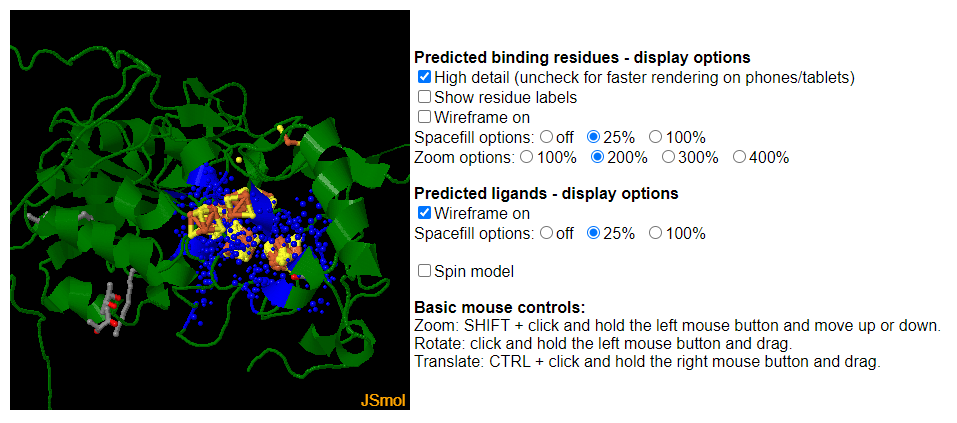
\includegraphics[width=\linewidth]{img/intfold_prediction.png}
    \caption{JSmol view of ligand binding residues prediction for T1114s2.
    Available at \url{https://www.reading.ac.uk/bioinf/servlets/nFOLD/IntFOLD7results.jsp?time=17_8_50_25_11-5-2022_CASP_ALL_mesu41b7re376c8l&md5=mesu41b7re376c8l&targetname=T1114s2}. The structure is shown in dark green, the binding sites prediction is shown in blue. Predicted ligands are shown yellow-orange. Available as a sample prediction from IntFOLD.}
    \label{fig:intfold_prediction}
\end{figure}

\subsection{COACH}

COACH\footnote{Available at \url{https://seq2fun.dcmb.med.umich.edu/COACH/}} is a web-based tool designed specifically for binding sites prediction, like PrankWeb. COACH uses a combination of substructure-comparison (TM-Site) and sequence-alignment (S-Site) methods for the computations \cite{yang2013protein}. These methods are generally slower than the P2Rank tool, so the prediction once again is available to the user after a longer time, typically around 24 hours. This tool allows the user not only to enter a FASTA sequence, but also to upload or paste a PDB file. COACH allows the user to download the prediction results as well and does not focus on the web visualization that is very limited. An example prediction is shown in Figure \ref{fig:coach_prediction}.

\begin{figure}
    \centering
    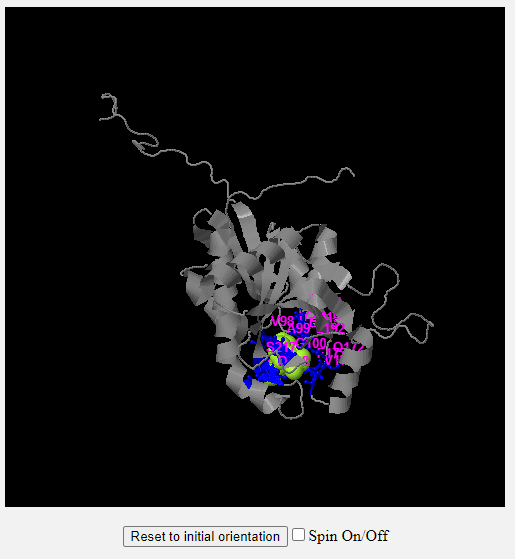
\includegraphics[width=.75\linewidth]{img/coach_prediction.png}
    \caption{JSmol view of a COACH prediction result for a sample protein available at \url{https://seq2fun.dcmb.med.umich.edu/COACH/CH000001/}. Compared to IntFOLD, the structure has implicitly less details and the user may change the representation only with a right mouse button click via JSMol settings.}
    \label{fig:coach_prediction}
\end{figure}

\subsection{DeepSite}

DeepSite\footnote{Available at \url{https://www.playmolecule.com/deepsite/}} is one of the newest tools for binding sites prediction. DeepSite is a part of PlayMolecule framework that aims at the visual representation of the protein structures and their interactions. DeepSite uses machine-learning based methods to precisely predict the binding sites, which makes the tool very fast \cite{10.1093/bioinformatics/btx350}. The waiting times are significantly slower and the prediction is available to the user after a few minutes. The user may enter the PDB structure ID, which is a lot more convenient way to describe the structure than by entering the entire PDB file. DeepSite utilizes the Mol* library for the results and is similar to PrankWeb in terms of the visual representation. On the other side, DeepSite provides the user only with a visualisation of the center of the binding site and does not provide any information about the residues that are involved in the binding directly in the web viewer. The structure is shown in a surface representation. An example prediction is shown in Figure \ref{fig:deepsite_prediction}. The pros of this tool are definitely the speed of the prediction and a above-average visual representation. On the other side, the user is provided with little information about the binding site and may be used for a rather quick overview of the potential binding sites.

\begin{figure}
    \centering
    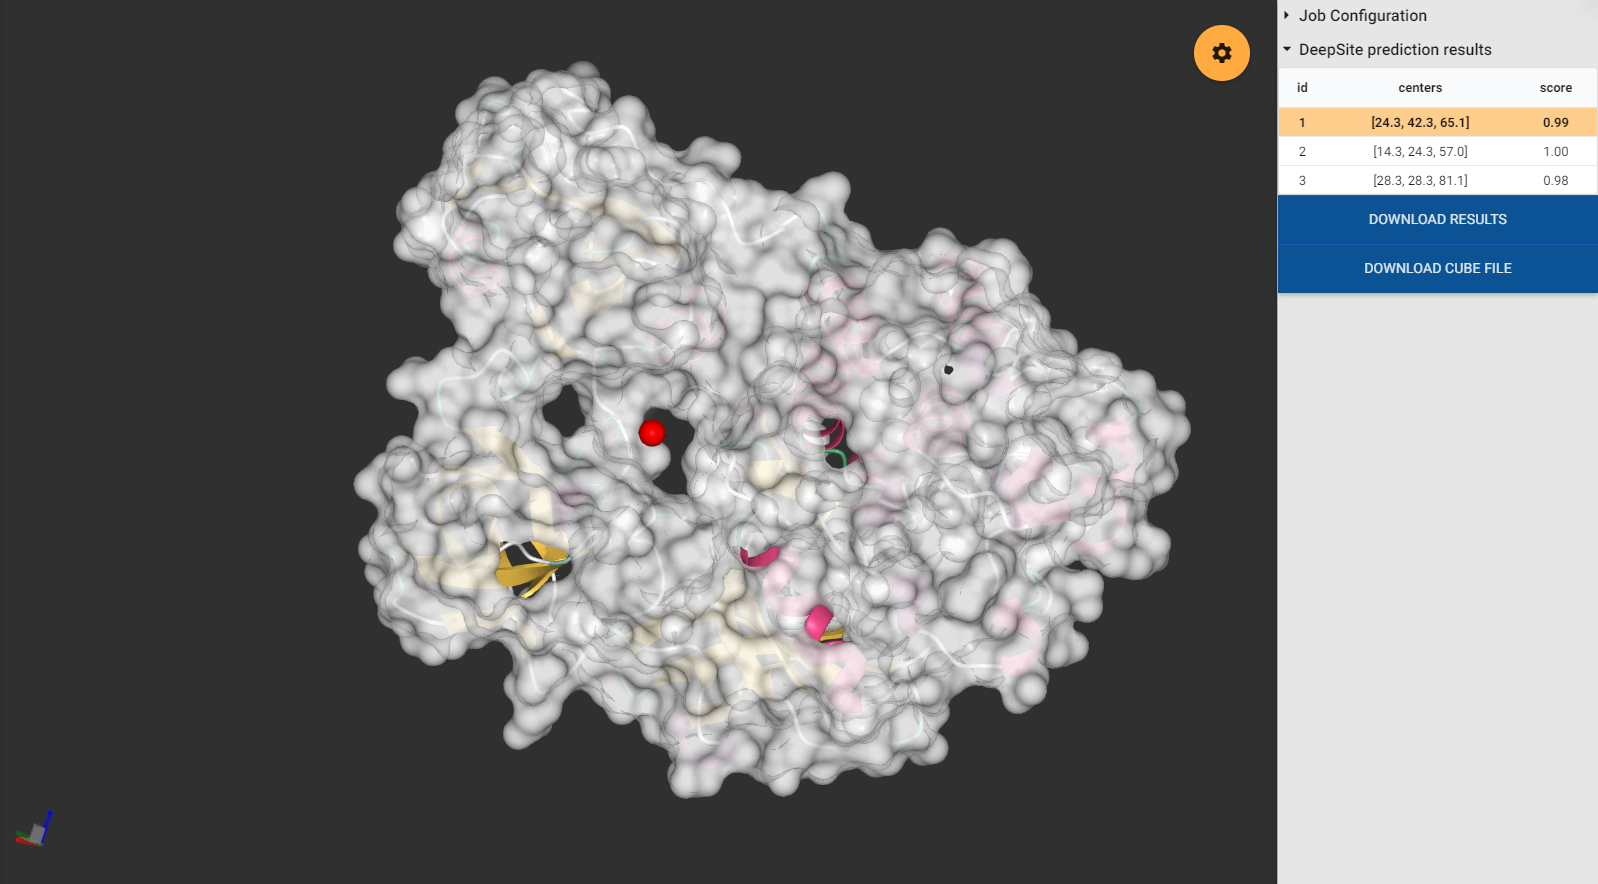
\includegraphics[width=\linewidth]{img/deepsite_prediction.png}
    \caption{A DeepSite prediction for the \texttt{2SRC} structure available at \url{https://www.playmolecule.com/deepsite/job/BD2ED307}. The surface representation is shown in white, underlying cartoon representation is colorful. The binding site prediction is shown by a red sphere.}
    \label{fig:deepsite_prediction}
\end{figure}

\xxx{todo}
\chapter{Programming documentation}
\label{chap:prog_docs}

This chapter will introduce the reader to the code changes made to the original PrankWeb interface. The first part will focus on the frontend, the second part will focus on the plug-ins.

\section{Frontend}
\label{sec:frontend}

The frontend of PrankWeb works as a TypeScript application. TypeScript is transpiled to JavaScript and bundled using Webpack. The application uses React for rendering a panel containing a tool box (see \cref{fig:toolbox}), structure information and pocket data. Styles are provided by CSS files and SCSS Bootstrap. All packages used in PrankWeb are installed using the npm tool. This architecture was already present in the original interface.

\begin{figure}[ht]
    \centering
    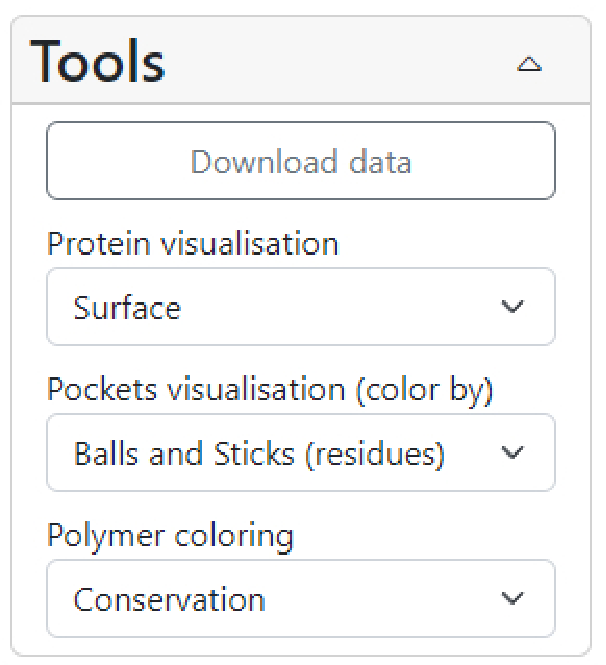
\includegraphics[width=0.4\linewidth]{img/toolsbox.pdf}
    \caption{The tool box component.}
    \label{fig:toolbox}
\end{figure}

The former interface was based on the LiteMol library for visualizing the structure. LiteMol is no longer developed, so one of the goals was to replace this plug-in with a new, modern structure viewer from the same authors - MolStar. Not only have the visuals significantly improved, the overall performance of MolStar is also much better. \cite{10.1093/nar/gkab314}

Before the current change, PrankWeb used a different library for rendering the 1D sequence visualization. The original implementation used the Protael library for a simple visual representation of the pockets, binding sites and scores. This library is intended for creating customizable visualizations for a protein structure \cite{10.1093/bioinformatics/btv605}. Protael is an old plug-in and in the original implementation, it needed to be modified in a significant way to fit the needs of PrankWeb. The new implementation presented in this thesis uses the RCSB Saguaro 1D Feature Viewer, which provides a more convenient way to display the pockets, binding sites and scores.

\subsection{High-level overview}
\label{subsec:frontend-overview}

Firstly, let's describe the typical data flow between the frontend and backend. Assuming that this section works with the \texttt{frontend} folder of the repository, this folder contains all of the frontend logic including plug-in configuration files for Webpack and static assets. The static assets are located in the \texttt{public} subfolder. Those include several libraries (such as jQuery), CSS files and static images.

Moving onto the visualization logic to the \texttt{viewer} subfolder, the user starts at the \texttt{index.js} page, where they enter either a protein structure file or a RCSB protein identifier. A request via REST API is then sent from the frontend to the backend workers. If there is a free worker, the job is immediately processed. If there are no free workers, the job is queued and processed as soon as a worker becomes available. The backend workers then process the job and create a result file (see \cref{subsec:executor-p2rank} for details). Right after the request, the user is redirected to the \texttt{analyze.ts} file. The frontend periodically fetches both the status file and the log file to display the current job progress. When the job is finished, the user is redirected to the \texttt{viewer.ts} file. The entrypoint to the viewer is the \texttt{renderProteinView} method, which will be covered later on. The viewer file is responsible for visualizing the structure, the pockets, binding sites and scores. The last step is to combine the plug-ins together, so that the user can interact with the structure and the data.

\subsection{MolStar}
\label{subsec:frontend-molstar}

MolStar (also Mol*) is a TypeScript library for visualizing protein structures. MolStar combines the strengths of the LiteMol and NGL libraries to provide a high-performance tool for bioinformatic scientists. The library is open-source and the code may be found on GitHub\footnote{https://github.com/molstar/molstar}. One downside of MolStar is that it lacks detailed documentation. There are some examples available in the GitHub repository either directly in the source codes or in issues, but for more complicated code, the user may need to create their own issue and ask the developers directly. An example of the visualization is shown in \cref{fig:molstar}.

\begin{figure}[htb]
    \centering
    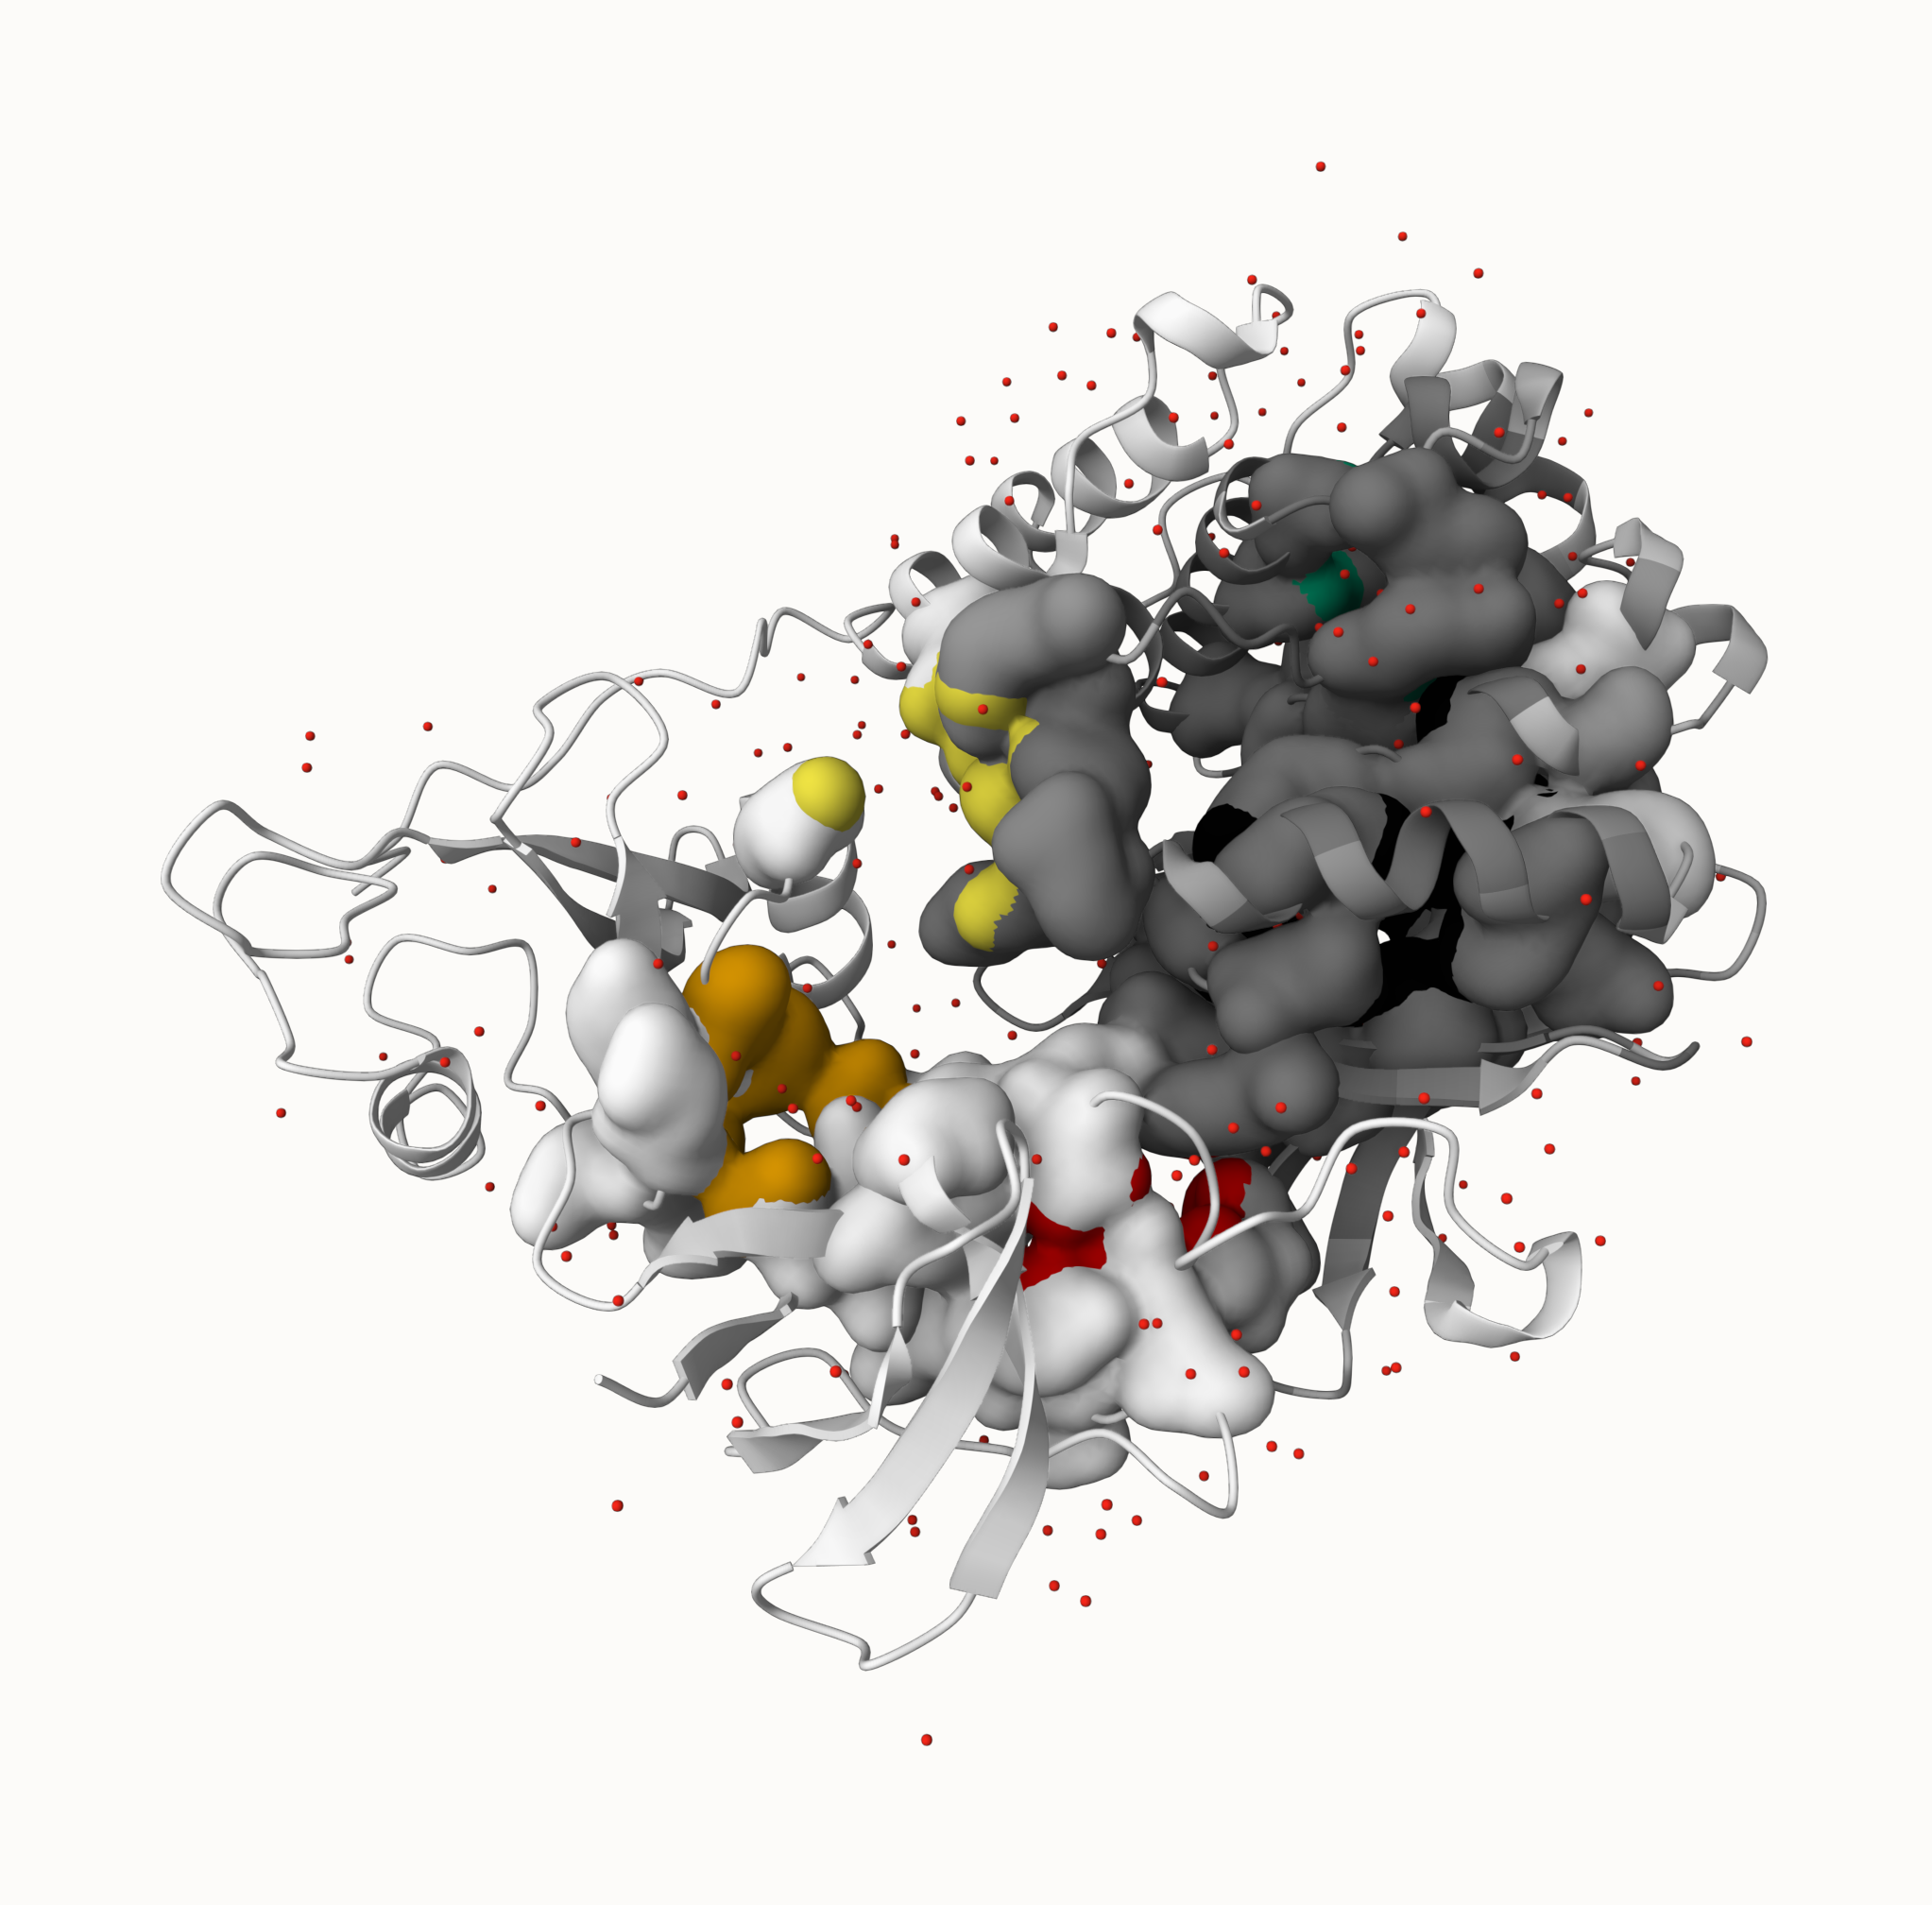
\includegraphics[width=\textwidth]{img/molstar_2src.png}
    \caption{A screenshot of the MolStar viewer for the \texttt{2SRC} structure. The structure is shown in cartoon representation and is colored by the conservation score. The pockets are shown in the surface representation.}
    \label{fig:molstar}
\end{figure}

After invoking the \texttt{renderProteinView} method, a MolStar viewer instance is created by calling the \texttt{createPluginUI} method from the library. An instance of \texttt{PluginUIContext} is returned. This instance is saved and used throughout the entire existence of the session. After the initialization, the main React component called \texttt{Application} is rendered for the first time. After mounting the component, the main visualization method \texttt{sendDataToPlugins} is called. This method from \texttt{data-loader.ts} is responsible for sending the prediction data for both plugins.

Some of the mentioned methods were already present in previous versions of PrankWeb. One of the goals of this thesis was to integrate MolStar into PrankWeb by replacing LiteMol. This lead to removal of the original LiteMol related code and introduced a few changes to the existing methods loading data into the viewer. All of MolStar related code was written from scratch to fit the needs of PrankWeb. Most of the code related to MolStar is located in the \texttt{molstar-visualise.ts} file. The following text describes the flow of the MolStar related interactions that create the core functionality of PrankWeb. These newly introduced methods call the MolStar library methods to create the visualization just from the data available in the prediction file and the structure file.

Firstly, the program asks for the API endpoint URL which resolves to a structure file. This file is loaded into MolStar via the \texttt{loadStructureIntoMolstar} method. This method parses the structure based on the file format and creates all of the available representations, such as surface, cartoon and ball-and-stick. It also tries to show the water molecules and ligands, if there are any.

When the structure is successfully shown to the user, a prediction is fetched from the API. Then, the 1D viewer is initialized. The 1D viewer connects to the MolStar plugin via callbacks. When the user hovers over a residue in the 1D viewer, the residue is highlighted in the MolStar plugin as well. When the user clicks a residue (or a pocket block), then the specific residue is focused in the MolStar plugin. The 1D viewer calls the \texttt{highlightInViewerAuthId} and \texttt{highlightInViewerLabelIdWithoutFocus} methods. See \cref{subsec:frontend-saguaro} for more details about the code that explains the interactions between the 1D viewer and the MolStar plugin.

After initializing the viewer and visualizing the structure, we need to show the pockets as well. The current implementation uses the following procedure: process every of the pockets and create a custom colored representation that will be added to the visualization. This is done in the \texttt{createPocketsGroupFromJson} method, which simply invokes \texttt{createPocketFromJson} for each of the pockets. That method creates multiple representations to allow the user to decide between various ways to display the pocket. Currently, a ball-and-stick and surface representations colored by either surface atoms or the entire residues are available. In future, more representations may be added. By default, only the surface atoms are shown as a pocket. The representations are added to a global variable containing all of them to allow switching between them based on user inputs from the React components.

For predicted structures, there is a special case. The predicted structure may contain areas that have not been properly analyzed, because no similar structures may be known. So, each of the resiudes is ranked with an AlphaFold pLDDT score that indicates how well a residue is predicted. Residues ranked with a score below 70 are ranked as low-confidence. \cite{jumper2021highly} PrankWeb enables the user to hide these residues from the visualization. This is done by creating a second structure visualization containing only the high-confidence residues. The user can switch between the two visualizations using a React component. For the creation of the second structure, we employ the \texttt{addPredictedPolymerRepresentation} method, which works in a similar way as creating the pockets.

After resolving the predicted structure, we have to ensure only the selected representations are visible to the user to ensure the best performance. This is done via the \texttt{showAllPocketsInRepresentation} method. Then, MolStar has to be linked to the 1D viewer, but in the opposite direction. Hovering over a residue in MolStar should highlight the corresponding residue in the 1D viewer. The method is called \texttt{linkMolstarToRcsb} and uses MolStar hover callbacks to achieve this behavior. The code is inspired by the MolArt library. \cite{molart}

In the last step, it is necessary to compute an average conservation (and potentially pLDDT) scores for each of the pockets. The JSON file provided by P2Rank contains the average scores only at the residue-level, so the pocket-level average needs to be computed. As we assume that the pockets are not large, this computation is done in the frontend and is not cached in any way. This is done in the \texttt{computePocketConservationAndAFAverage} method.

In this step, the MolStar visualization is complete and ready-to-use. The user may interact with the structure either via the 1D viewer, or via the MolStar plugin, or via the React components. The last part of the code is responsible for enabling interactions with the React tools. Currently, the user may interact with MolStar from the components in the following ways:

\begin{itemize}
    \item Change structure representation
    \item Change pockets representation
    \item Color residues by conservation or pLDDT scores
    \item Hide low-confidence residues for predicted structures
    \item Hide/show all pockets
    \item Hide/show individual pockets
    \item Highlight a pocket including zoom
\end{itemize}

All of the interactions are handled by calling the respective methods directly from the React components, which are described in \cref{subsec:frontend-react}. We will not cover details of the code, as it is mostly straightforward and the code is documented. The main idea is to apply transforms to the MolStar structure which is then re-rendered by the library.

In the end, we will show a brief code structure of the \texttt{molstar-visualise.ts} file containing the vast majority of MolStar-related code, just to give an overview of the MolStar integration.

\lstinputlisting[language=JavaScript,caption={
    A slightly edited version of a declaration file \texttt{molstar-visualise.d.ts}.
}]{code/molstar-visualise.d.ts}


\subsection{RCSB Saguaro 1D Feature Viewer}
\label{subsec:frontend-saguaro}

Alongside to the MolStar plugin, we use the RCSB Saguaro 1D Feature Viewer to display the pockets, actual binding sites and scores in a simple view mapped to the residues, which is the key feature of this plugin. The viewer is designed to easily identify multiple annotations on a single residue.

The RCSB Saguaro 1D Feature Viewer is a TypeScript library for visualizing protein features in a 1D view. An example usage is shown in \cref{fig:1d-viewer}. The code is available on GitHub\footnote{\url{https://github.com/rcsb/rcsb-saguaro}}. Documentation is available and the usage is simple, but it is important to keep in mind that the library is still under active development and the interface may change in the future.

\begin{figure}[htb]
    \centering
    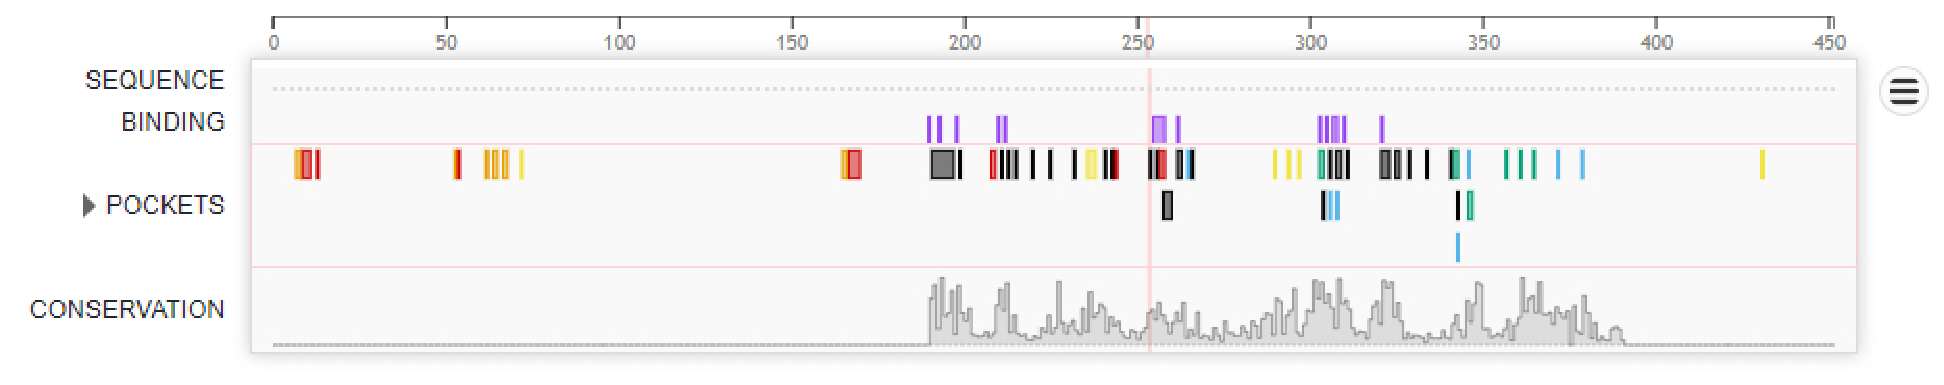
\includegraphics[width=\linewidth]{img/rcsb_2src.pdf}
    \caption{The RCSB Saguaro 1D Feature Viewer for the \texttt{2SRC} structure.}
    \label{fig:1d-viewer}
\end{figure}

In the original PrankWeb implementation, Protael was used for mapping the annotation to the single residues. In this thesis, we decided to use the RCSB Saguaro 1D Feature Viewer instead. The main reason for this decision is that the RCSB Saguaro 1D Feature Viewer is a more extensible library and is actively maintained. So, all of the code related to Protael was removed and replaced with new code using the RCSB Saguaro 1D Feature Viewer to provide the same functionality.

Most of the methods are defined in the \texttt{rcsb-visualise.ts} file. In our case, as described in \cref{subsec:frontend-molstar}, the 1D viewer gets initialized by the \texttt{sendDataToPlugins} method. This calls the \texttt{initRcsb} method which prepares all of the data for the plug-in.

The first thing to notice is calculating the viewer actual width. This is done in the \texttt{calculateViewerWidth} method. Unluckily, the viewer allows only a fixed width measured in pixels. This is a problem, as the viewer is not responsive and every time the user resizes the window, the viewer would have to be re-initialized, which would be pretty inefficient. So, for the first time the page loads, we calculate the width of the viewer based on a knowledge of the desired width that is set via CSS. We also have to subtract a certain amount of pixels to account not only for the viewer itself, but also for the margins, paddings and a custom viewer scrollbar, which is, once again, in-built in the viewer and is not customizable. We discussed this issue and came to a conclusion that the best solution is to add better-looking custom scrollbars to the viewer to provide a better user experience until the viewer is made responsive.

Then, the RCSB board is configured to interact with the MolStar viewer. This is done via the \texttt{onHighlight} and \texttt{elementClicked} methods. The first method is called when the user hovers over a certain residue in the 1D viewer. The actual callback is debounced to prevent lagging. A request for highlighting the specific residue in MolStar is then sent. The second method is called when the user clicks on a residues in the 1D viewer. A similar request is sent to MolStar with the difference that the residue is also zoomed in.

The last step is to prepare the actual data for each of the so-called tracks. A track represents one row (or multiple rows) containing information about a specific annotation. This is done in the \texttt{createRowConfigDataRcsb} method. A sequence track simply contains the protein amino acids. The binding track contains the actual binding sites computed by P2Rank. Pocket tracks are distinguished by different colors, which are picked firstly based on color-blind schemes to ensure the best accessibility, secondly randomly. The pocket color is changed in the original pocket data as well, so that the same colors for the pockets are used throughout the application. The last tracks are the conservation and pLDDT tracks, if available. Computation of the pocket tracks is not simple and straightforward, as the JSON file provided by P2Rank does not fit the viewer's interface, so the method highly relies on the JSON structure.

The 1D viewer does not rely on any React components and the only interaction may be done via the MolStar plugin simply by hovering over the residues, as described in \cref{subsec:frontend-molstar}.

Similarly to MolStar, let's have a look at the \texttt{rcsb-visualise.ts} file structure and the most important methods.

\lstinputlisting[language=JavaScript,caption={
    A slightly edited version of a declaration file \texttt{rcsb-visualise.d.ts}.
}]{code/rcsb-visualise.d.ts}


\subsection{React components}
\label{subsec:frontend-react}

This section will describe the React components that are related to the structure visualization. Most of the components were already present in the previous version of PrankWeb, but there was a need to refactor them to make them more modular and reusable, as well as to add new features and improve the user experience.

The application uses the following components:

\begin{itemize}
    \item \textbf{Application} - the main component of the app, responsible for the overall structure of the page including the viewers
    \item \textbf{ToolBox} - a component containing tools for changing the structure representation, coloring residues, hiding low-confidence residues and downloading data
    \item \textbf{StructureInformation} - a component containing the structure name
    \item \textbf{PocketList} - a component containing a list of all pockets with their scores and a button for hiding/showing all of them
    \item \textbf{Pocket} - a component containing a single pocket with its information and buttons for hiding/showing the pocket, highlighting the pocket and opening a dialog with the pocket details
    \item \textbf{PocketDetails} - a component defining the information of a Pocket component
    \item \textbf{PocketProperty} - a component visualizing a single property of a Pocket component
\end{itemize}

Other components will be covered in \cref{sec:plugins} as they are related to the plug-ins.

All React components are defined in their own files in the \texttt{components} subdirectory. The components extend the \texttt{React.Component} class to utilize the props and state features of React. The components invoke the responsible RCSB and MolStar methods on various value changes, clicks on buttons and other events. Some of the props get passed from the parent component to the children, which allows an easy communication between them and enforces best practices and minimizes code duplication. Some of the components have state variables as well that mostly indicate their current visibility. The components create a tree that is visualized in \cref{fig:react-molstar}.

The components are styled as Bootstrap cards and thus they are responsive. Although we expect the user to use PrankWeb mainly on a desktop computer, it is necessary to provide a good first experience when encountering the application on a smaller screen.

\xxx{TODO: add UML diagram}

\begin{figure}[htb]
    \centering
    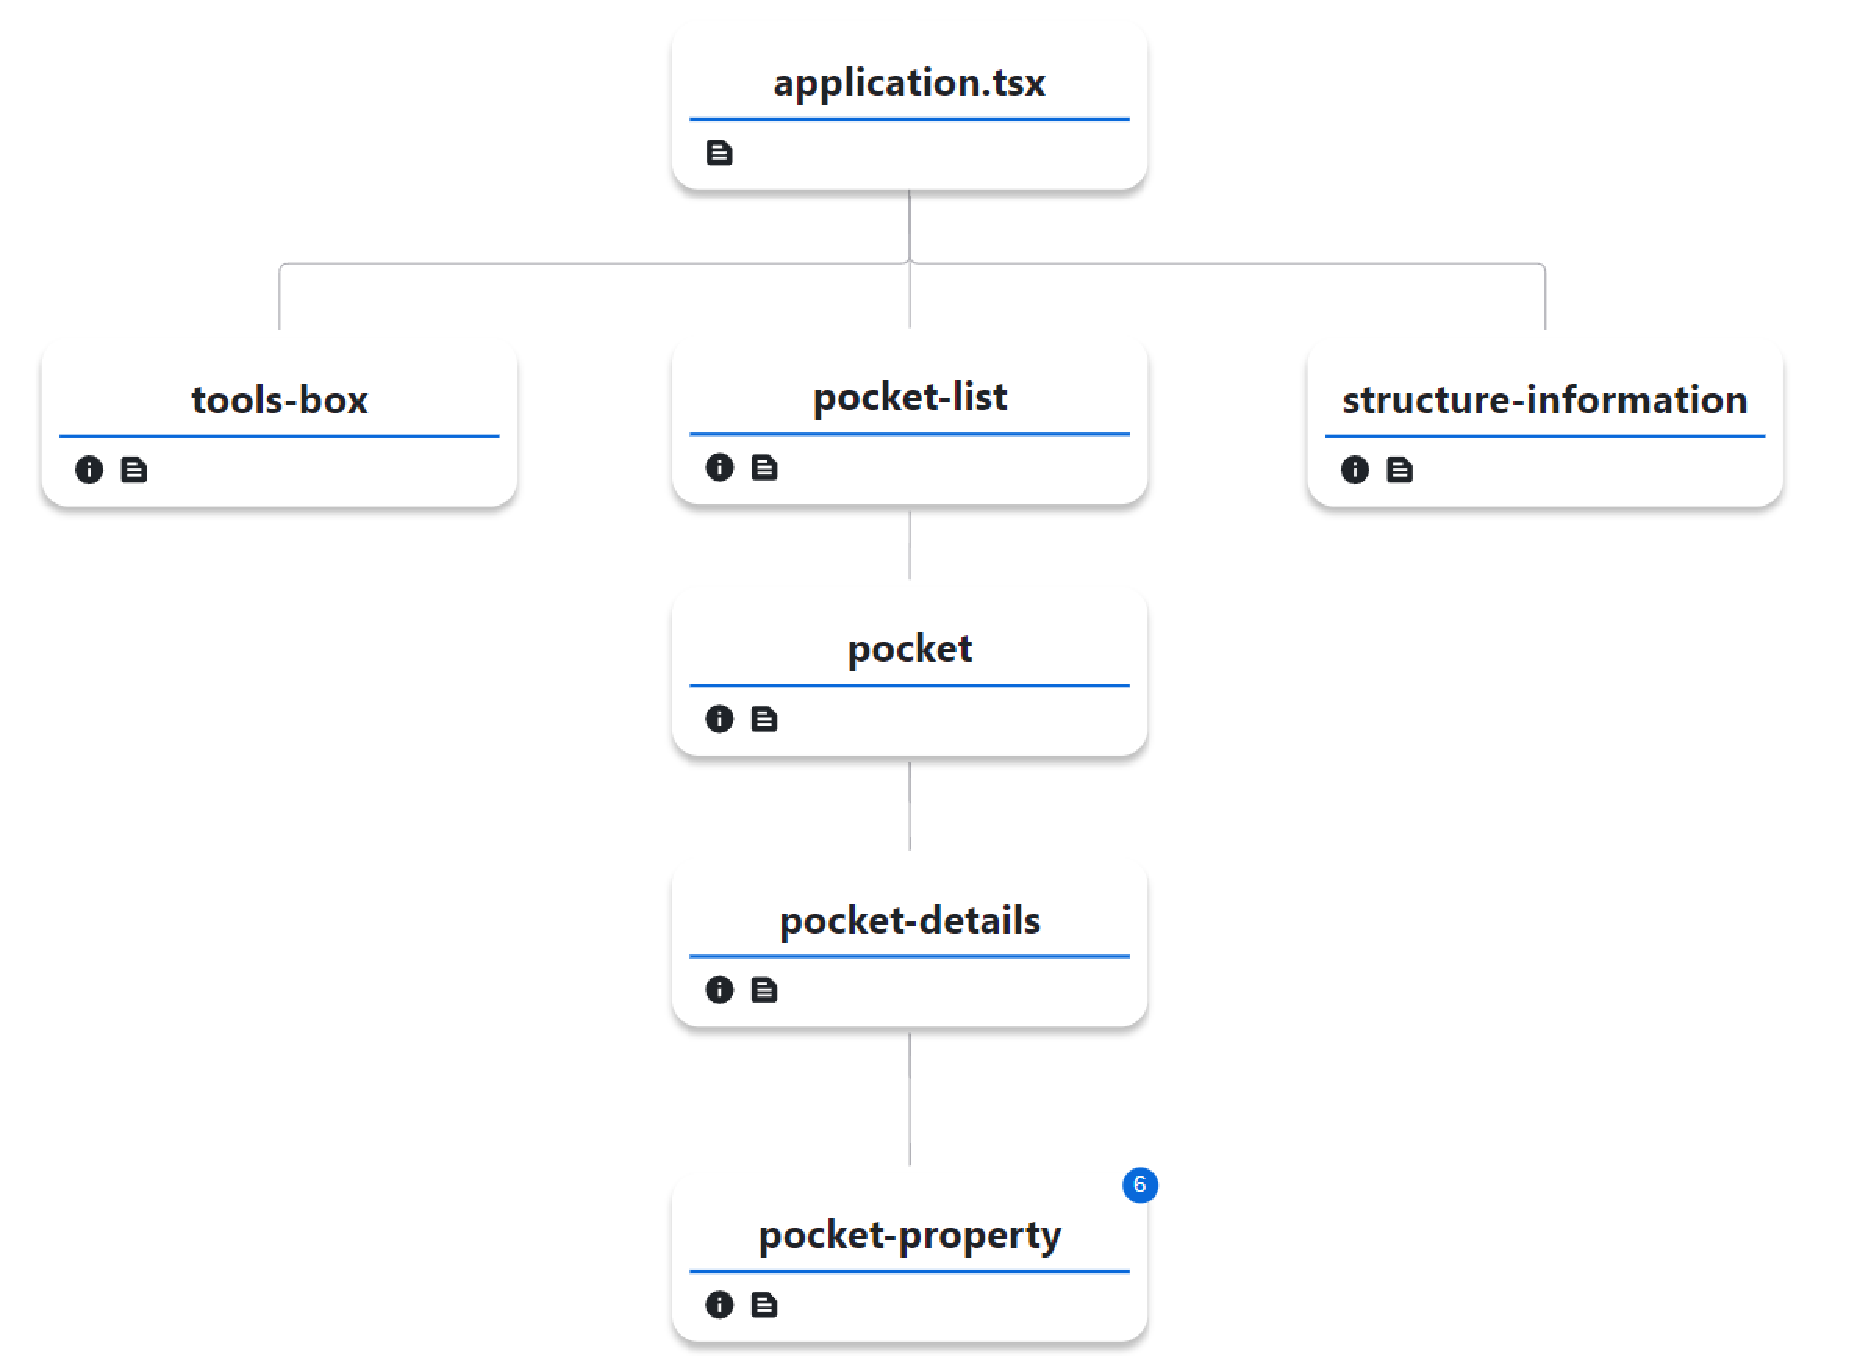
\includegraphics[width=\textwidth]{img/react_molstar.pdf}
    \caption{The React component tree showing only the components that are not related to the plug-ins.}
    \label{fig:react-molstar}
\end{figure}

\section{Plug-ins}
\label{sec:plugins}

The second goal of this thesis was to introduce a possibility to extend the current functionality of the application by adding new plug-ins (also called tasks, these terms are used interchangeably). The plug-ins enable post-proccesing of the pockets. 

After a discussion, we created the following plug-in categories: client-side and server-side. It is assumed that the client-side plug-ins will be used for simpler tasks that may be computed from the existing data in each session, on the contrary the server-side plug-ins will be used for complex tasks that are more time-consuming and possibly utilize third-party software.

The PrankWeb interface for both of the tasks works as a set of React components that are modular, so new plug-ins may be introduced in an easy way without modifying much of the current code.

For an easy access to plug-ins, we have created a possibility to view the pocket details not only directly in the pocket list, but in a draggable dialog as well. This dialog is defined in the \texttt{DraggableDialog} and \texttt{PocketDialogDetails} classes that provide the implementation. The user may open multiple dialogs at once as well as drag them around the screen. The dialogs allow interaction behind them, so the user may still manipulate with both of the viewers.

This decision was discussed more and multiple designs were proposed and tested. All of the possible variants are listed in \cref{sec:pocket_detail_designs}. The final decision was made based on the fact that a vast majority of users is expected to use a big-screen device, so to keep the original usage easy and intuitive, we decided to keep the original design. One downside of this implementation is that the dialogs are not intended to be used on mobile devices. In other words, the dialogs are not available for small screens which makes this section irrelevant for those devices. On the other side, we believe that this is a reasonable trade-off.

In the following subsections, we will introduce the general plug-in interface and the implemented plug-ins.

\subsection{Client-side plug-ins}
\label{subsec:client-side-plugins}

The main intention of client-side plug-ins is to create a possibility to enable simple post-processing from the prediction data directly in the application. The tasks computed on client-side stay in the current session. 

Currently, the client-side plug-ins are defined in a \texttt{PocketDialogDetails} component as they are dialog-specific. A new interface for these plug-ins was created in the \texttt{PocketClientTask} component. Let's have a look at the interface.

\lstinputlisting[language=JavaScript,caption={
    An edited version of the \texttt{pocket-client-task.tsx} component.
}]{code/pocket-client-task.tsx}

Some of the props and state variables are self-explanatory, some of them are passed from the parent component. We will focus on the client-side specific props and state variables that define their behavior.

Firstly, let's take a look at the \texttt{taskType} prop. This prop defines the type of the task that is defined in the \texttt{ClientTaskType} enum. This enables a possible behavior difference of the client-side plug-ins based on their type. Next prop is a method called \texttt{compute}. This is the key method of the plug-in that provides the actual post-processing of the prediction data. The behavior is defined by the parent component. In the plug-in definition, the \texttt{compute} method is called. We expect this method to return a promise containing data conforming to the \texttt{ClientTaskData} interface. After receiving the result, the result needs to be rendered. During this entire process, state variables \texttt{taskData}, \texttt{computed} and \texttt{loading} are used to indicate the current computation progress.

Originally, one implementation for showing the result was created, but to provide a more generic approach to the problem, a second method was introduced to the props - the \texttt{renderOnComplete} method. This method takes the computed data as a parameter and returns a JSX component that renders the data inside the original dialog.

Currently, the client-side plug-ins are defined in the \texttt{tasks} subdirectory. The actual implementations are \texttt{.tsx} files and should contain both of the methods for the computation and rendering to keep the code clean.

As an example of a client-side plug-in, we have implemented a plug-in that computes the expected volume of the pocket. For this purpose, we have created a \texttt{tasks/client-atoms-volume.tsx} file that contains \texttt{computePocketVolume} and \texttt{renderOnTaskVolumeCompleted} methods that conform to the \texttt{compute} and \texttt{renderOnComplete} props of the \texttt{PocketClientTask} component. In this post-processing, we are using a convex hull algorithm to get coordinates of the hull vertices. Then, we use a simple formula to compute the volume of the convex hull using the coordinates of the vertices based on triangulation of the hull \cite{zhang2001efficient}. The result is then rendered in the dialog as a simple number. This implementation saves the computed results in a hashmap directly in the implementation file. This is not the most efficient way to store the results, on the other hand, it is a simple solution that is sufficient for this use case.

Creating a custom new client-side plug-in is covered in detail in \cref{sec:developer}.

\subsection{Server-side plug-ins}
\label{subsec:server-side-plugins}

Server-side plug-ins create an opportunity to perform more complex post-processing that takes more time to compute. Our intention was to allow users to use third-party software for the post-processing. Server-side tasks are meant to be parametrized by the user in some way.

The plug-ins are defined in a similar way as the P2Rank executor, which may be processed by Docker containers (as mentioned in \cref{sec:prankweb_arch}).

There are a few steps that have to be done to implement a new server-side plug-in. First, API endpoints for the plug-in as well as the folder and file structure need to be defined. This is done in the \texttt{web-server} folder in Flask. Usually, it is expected that Flask will prepare the needed directories and files for the actual Docker container. For this process, it is typical to create a new Python class to contain all of this logic.

Then, in the Celery client configuration file in Flask, new bindings are created for the new plug-in. This includes creating a new Celery queue as well as introducing a new task that gets executed on the backend identified by its name.

After completing all of the Flask tasks, a new Docker container has to be created. The container should install Python with Celery and any other tools needed for the post-processing. It is expected that a new \texttt{Dockerfile} will be created for this purpose. After setting up the container, Celery bindings have to be created in a similar way as in Flask. Then, any method may be called from this Celery binding. This means that the actual post-processing may be finally done here. The first option is to do this in Python entirely, but it is also possible to call any other tool from the container. The only requirement is to have everything set up properly. 

The Docker container is also responsible for saving the results of the post-processing. This means that either some of the Python files or the third-party tool itself has to save the results in the correct location. Keep in mind that the location is very likely to depend on the API endpoints defined in Flask. Now, the Docker container is ready to be used.

It is highly recommended to include the newly created container into the Docker-compose file. This makes the deployment easy and allows simpler testing of the new plug-in\footnote{With Docker-compose, it is possible to restart just one of the containers, which makes the debugging faster.}.

After completing all of the steps, the new plug-in should be ready to be used. The only thing left is to include the plug-in to the frontend. For the frontend interaction, a new React component was introduced.

\texttt{PocketServerParametrizedTask} is meant to be used for the server-side plug-ins that require some parameters to be set by the user. This component is used in \texttt{PocketDialogDetails} similarly to client plug-ins (more about dialog in \cref{subsec:client-side-plugins}). Let's have a look at the server plug-in component.

\lstinputlisting[language=JavaScript,caption={
    An edited version of the \texttt{pocket-server-parametrized-task.tsx} component.
}]{code/pocket-server-parametrized-task.tsx}

The component works similarly to the client-side plug-in component. There are two methods that are responsible for the computation and rendering of the results. One of the differences is that these two methods are now identifiable by a hash that has to be computed from the parameters before the actual computation. The computation of a hash is done via the \texttt{hashMethod} method. This hash is not only used for frontend identification, but also for the backend. It is up to the developer, whether they will consider it as a possible input or just as a string for identification. This technique allows us to differ between multiple tasks of the same type with different parameters.

There are more state variables as well. \texttt{modalOpen} and \texttt{formData} were introduced for receiving an input from the user, the current implementation opens a modal dialog with a text area. The \texttt{hash} is then computed from the input stored in the \texttt{formData} variable.

As the task results are persistent on the server, a new variable called \texttt{serverTasks} was introduced in the main component of the app. This component then periodically checks for all computed tasks for the given structure. The objects in this array are mutable and are modified for the purpose of the frontend rendering, so only the response data for tasks completed in this session are saved.

This allows us to render the hashes of the tasks that were computed both in this session and in previous ones. For this purpose, a new component called \texttt{TaskList} was introduced to display the list of tasks. \xxx{TODO: maybe we won't use this component in the end, so mention that its just available but not used}

One last change was made to the \texttt{PocketDialogDetails} component. A new component \texttt{PocketRunningTasks} was created to display a list of tasks that are either running or completed in this session. This is done to make sure that the task results are available to the user in case the dialog is closed and reopened. Moreover, this allows the user to enter multiple parameters for the same task and see the results for all of them.

One of the goals of this thesis was to implement basic \textbf{server-side molecular docking}. Docking may be computationally very demanding, this makes it a perfect candidate for a server-side plug-in.

Firstly, we designed a public API for the docking requests. There were three main needs:
\begin{enumerate}
    \item Starting new docking task with a given user input.
    \item Receiving task results.
    \item Receiving information about all tasks (including their status).
\end{enumerate}
The API routes were added to the Flask configuration file. The routes are defined as follows:

\lstinputlisting[language=Python,caption={
    An edited version of the \texttt{api\_v2.py} file.
}]{code/api-v2.py}

After designing the routes, a new class called \texttt{DockingTask} was created. This class is responsible for serving the API requests. This includes definition of the directory structure, saving the input files, preparing the info file, and calling the actual docking tool on the backend. In this class, most of the file errors are handled, as there are many opportunities for wrong inputs and requests. As all of the methods are important, we will focus on the one that is responsible for the actual docking. That is the \texttt{submit\_directory\_for\_docking} defined in the Celery client configuration file. This method sends a task named \texttt{docking} to the Celery queue. Note that for docking, a new Celery queue was created in the configuration file.

\lstinputlisting[language=Python,caption={
    An edited version of the \texttt{celery\_client.py} file.
}]{code/celery-client.py}

Then, a new Docker container was created in the \texttt{executor-docking} directory and added to the Docker-compose files. We introduced a new Docker volume to preserve the results as well. An important part of this step is to mark this container with the right Celery queue in the command.

\lstinputlisting[language=clean,caption={
    An edited extract from the \texttt{docker-compose.yml} file.
}]{code/docker-compose.yml}

The newly created Docker container is described in the \texttt{Dockerfile}. All of the needed tools for docking are downloaded and set up there. After setting up the container, Celery bindings are created in a similar way as in Flask in the \texttt{celery\_docking.py} file. This file contains routing for the Celery task sent from the Flask server. This calls methods from \texttt{run\_task.py} that contains that handle all of the work with the info file for the given structure (updates the status and timestamps). From there, the \texttt{dock\_molecule} method is called. \texttt{dock\_molecule} is responsible for the actual docking.

Firstly, the structure is unzipped from the gzipped file created during the initial prediction. Then, we treat \texttt{.pdb} files a bit differently, structures in this file format are cleaned using the lePro tool to remove unnecessary information. After the possible structure cleanup, a tool called \texttt{prepare\_receptor} from the ADFR Suite to prepare the structure for docking. \cite{ravindranath2015autodockfr} Moving on, ligand preparation is done using the \texttt{rdkit} and \texttt{meeko} Python packages. \cite{landrum2013rdkit} The last step before docking is to prepare the bounding box for the docking program. This is done manually by parsing the input file, saving the result to a text file.

In this stage, everything is properly set up for the docking. We use the \texttt{AutoDock Vina} program for the docking. AutoDock Vina enables us to dock the ligand in a simple and fast way, on the other side, the results are not as accurate. \cite{trott2010autodock} We still decided to use this tool due to a rather simple setup and fast computation. The docking program is invoked with the prepared parameters and the results are saved to a public folder.

After the docking, the info file is updated with the result. The result file then may be downloaded by the actual user. The file may be viewed in several tools, such as PyMOL.

Now, the only thing left is to implement the frontend components to provide an user-friendly way to dock the molecules. We created a \texttt{ServerTaskData} enum for potential, alongside to \texttt{ServerTaskDataContents} that is an interface for data from the server-side. The main logic of server-side plugins is defined by implementing the \texttt{PocketServerParametrizedTask} component that was added to the \texttt{PocketDialogDetails} component in a similar way to the client plug-ins (see \cref{subsec:client-side-plugins}). The implementation was done in the \texttt{tasks/server-docking-task.tsx} file. This file has private methods that compute a bounding box for docking before submitting the task, and public exported methods that are responsible for calling the API and displaying the results. One of the methods should hash the input, but as long as we are using SMILES molecule representation \cite{weininger1988smiles}, there is no need to hash the input.

To finish the frontend implementation, a few more components are updated in order to show all results correctly. Firstly, we modified the \texttt{Application} component to keep all of the docking tasks in its state variable. This is done in the \texttt{getTaskList} method to create an ability to show all results of the completed tasks in the current session. This state variable called \texttt{serverTasks} then propagates to other components. Lastly, we bound the previously created methods to the \texttt{PocketRunningTasks} component to display the results of the docking tasks in the dialog window.

Creating a custom new server-side plug-in is briefly described in \cref{sec:developer}.

\chapter{User documentation}
\label{chap:user_docs}

\xxx{TODO: add motivation for users, distinguish between a regular user and a developer}

\section{Deployment}
\label{sec:deployment}

This section describes how to deploy the application. The preffered way is to deploy PrankWeb using Docker. Local development and deployment is limited.

\subsection{Docker deployment}
\label{subsec:docker_deployment}

Firstly, Docker and Docker Compose need to be installed\footnote{Downloadable from the official website at \url{https://docs.docker.com/get-docker/}}. 

After installing Docker, the PrankWeb repository needs to be cloned, preferrably using Git\footnote{Downloadable from the official website at \url{https://git-scm.com/downloads}}.

\begin{enumerate}
    \item Create a directory for the PrankWeb repository and navigate to it.
    \item Clone the repository using the following command:
    \begin{lstlisting}
        git clone https://github.com/cusbg/prankweb.git .
    \end{lstlisting}
    \item Create directories for each of the volumes.
    \item Create mounts for each of the volumes in the \texttt{docker-compose.yml} file. The mounts are created as follows, simply update the \texttt{/tmp/} paths to the paths of the directories created in the previous step:
    \begin{lstlisting}
        docker volume create --name prankweb_rabbitmq --opt type=none --opt device=/tmp/rabbitmq --opt o=bind

        docker volume create --name prankweb_conservation --opt type=none --opt device=/tmp/conservation --opt o=bind

        docker volume create --name prankweb_predictions --opt type=none --opt device=/tmp/predictions --opt o=bind

        docker volume create --name prankweb_services --opt type=none --opt device=/tmp/services --opt o=bind
    \end{lstlisting}
    \xxx{TODO: maybe add docking}
    \item Optionally, create a \texttt{.env} file to change the default variables defined in the \texttt{docker-compose.yml} file. Notice that UID and GID need to have write permissions to the directories created in the previous steps.
    \item Build the Docker images using the following command:
    \begin{lstlisting}
        docker-compose build
    \end{lstlisting}
    \item Optionally, download the conservation database (keep in mind that this database is large, around 30 GB):
    \begin{lstlisting}
        docker-compose run --rm executor python3 /opt/hmm-based-conservation/download_database.py
    \end{lstlisting}
    \item Start the containers using the following command:
    \begin{lstlisting}
        docker-compose up
    \end{lstlisting}
\end{enumerate}

The application is now be accessible at \url{http://localhost:8020/}.

Although the main deployment process will not change much, the best way to get the current information is to refer to the official documentation at \url{https://github.com/cusbg/p2rank-framework/wiki/PrankWeb-deploy-with-Docker}.

\subsection{Local deployment}
\label{subsec:local_deployment}

\xxx{TODO: how to deploy via Docker}

\section{Regular user}
\label{sec:regular_user}
\xxx{TODO: add some screenshots and a brief description of the UI}

\section{Developer}
\label{sec:developer}
\xxx{TODO: add a brief description on how to add new client/server side tasks, change the current visuals etc.}

\chapter{More complicated chapter}
\label{chap:math}

After the reader gained sufficient knowledge to understand your problem in xyz, you can jump to your own advanced material and conclusions.

You will need definitions (see \cref{defn:x} below in \cref{sec:demo}), theorems (\cref{thm:y}), general mathematics, algorithms (\cref{alg:w}), and tables (\cref{tab:z})\todo{See documentation of package \texttt{booktabs} for hints on typesetting tables. As a main rule, \emph{never} draw a vertical line.}. \Cref{fig:f,fig:g} show how to make a nice figure. See \cref{fig:schema} for an example of TikZ-based diagram. Cross-referencing helps a lot to keep the necessary parts of the narrative close --- use references to the previous chapter with theory wherever it seems that the reader could have forgotten the required context.

\section{Example with some mathematics}
\label{sec:demo}

\begin{defn}[Triplet]\label{defn:x}
Given stuff $X$, $Y$ and $Z$, we will write a \emph{triplet} of the stuff as $(X,Y,Z)$.
\end{defn}

\newcommand{\Col}{\textsc{Colour}}

\begin{thm}[Car coloring]\label{thm:y}
All cars have the same color. More specifically, for any set of cars $C$, we have
$$(\forall c_1, c_2 \in C)\:\Col(c_1) = \Col(c_2).$$
\end{thm}

\begin{proof}
Use induction on sets of cars $C$. The statement holds trivially for $|C|\leq1$. For larger $C$, select 2 overlapping subsets of $C$ smaller than $|C|$ (thus same-colored). Overlapping cars need to have the same color as the cars outside the overlap, thus also the whole $C$ is same-colored.\todo{This is plain wrong though.}
\end{proof}

\begin{table}
% uncomment the following line if you use the fitted top captions for tables
% (see the \floatsetup[table] comments in `macros.tex`.
%\floatbox{table}[\FBwidth]{
\centering\footnotesize\sf
\begin{tabular}{llrl}
\toprule
Column A & Column 2 & Numbers & More \\
\midrule
Asd & QWERTY & 123123 & -- \\
Asd qsd 1sd & \textcolor{red}{BAD} & 234234234 & This line should be helpful. \\
Asd & \textcolor{blue}{INTERESTING} & 123123123 & -- \\
Asd qsd 1sd & \textcolor{violet!50}{PLAIN WEIRD} & 234234234 & -- \\
Asd & QWERTY & 123123 & -- \\
\addlinespace % a nice non-intrusive separator of data groups (or final table sums)
Asd qsd 1sd & \textcolor{green!80!black}{GOOD} & 234234299 & -- \\
Asd & NUMBER & \textbf{123123} & -- \\
Asd qsd 1sd & DIFFERENT & 234234234 & (no data) \\
\bottomrule
\end{tabular}
%}{  % uncomment if you use the \floatbox (as above), erase otherwise
\caption{An example table.  Table caption should clearly explain how to interpret the data in the table. Use some visual guide, such as boldface or color coding, to highlight the most important results (e.g., comparison winners).}
%}  % uncomment if you use the \floatbox
\label{tab:z}
\end{table}

\begin{figure}
\centering
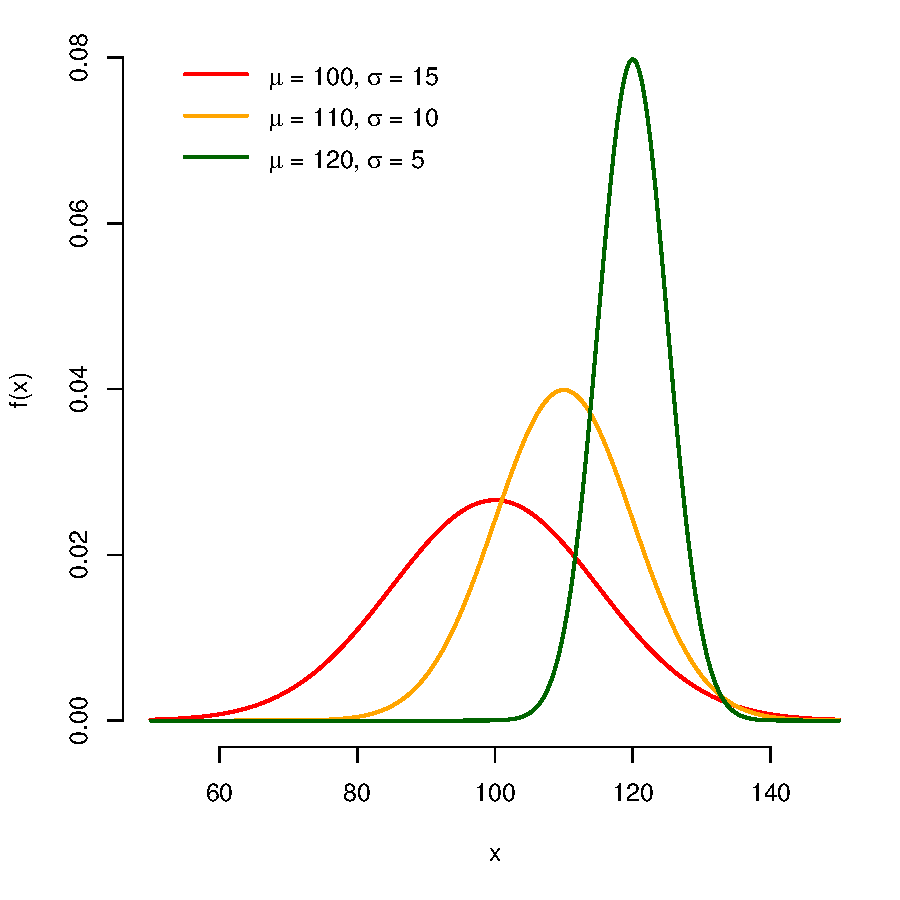
\includegraphics[width=.6\linewidth]{img/ukazka-obr02.pdf}
\caption{A figure with a plot, not entirely related to anything. If you copy the figures from anywhere, always refer to the original author, ideally by citation (if possible). In particular, this picture --- and many others, also a lot of surrounding code --- was taken from the example bachelor thesis of MFF, originally created by Martin Mareš and others.}
\label{fig:g}
\end{figure}

\begin{figure}
\centering
\tikzstyle{box}=[rectangle,draw,rounded corners=0.5ex,fill=green!10]
\begin{tikzpicture}[thick,font=\sf\scriptsize]
\node[box,rotate=45] (a) {A test.};
\node[] (b) at (4,0) {Node with no border!};
\node[circle,draw,dashed,fill=yellow!20, text width=6em, align=center] (c) at (0,4) {Ugly yellow node.\\Is this the Sun?};
\node[box, right=1cm of c] (d) {Math: $X=\sqrt{\frac{y}{z}}$};
\draw[->](a) to (b);
\draw[->](a) to[bend left=30] node[midway,sloped,anchor=north] {flow flows} (c);
\draw[->>>,dotted](b) to[bend right=30] (d);
\draw[ultra thick](c) to (d);

\end{tikzpicture}
\caption{An example diagram typeset with TikZ.}
\label{fig:schema}
\end{figure}

\begin{algorithm}
\begin{algorithmic}
\Function{ExecuteWithHighProbability}{$A$}
	\State $r \gets$ a random number between $0$ and $1$
	\State $\varepsilon \gets 0.0000000000000000000000000000000000000042$
	\If{$r\geq\varepsilon$}
		\State execute $A$ \Comment{We discard the return value}
	\Else
		\State print: \texttt{Not today, sorry.}
	\EndIf
\EndFunction
\end{algorithmic}
\caption{Algorithm that executes an action with high probability. Do not care about formal semantics in the pseudocode --- semicolons, types, correct function call parameters and similar nonsense from `realistic' languages can be safely omitted. Instead make sure that the intuition behind (and perhaps some hints about its correctness or various corner cases) can be seen as easily as possible.}
\label{alg:w}
\end{algorithm}

\section{Extra typesetting hints}

Do not overuse text formatting for highlighting various important parts of your sentences. If an idea cannot be communicated without formatting, the sentence probably needs rewriting anyway. Imagine the thesis being read aloud as a podcast --- the storytellers are generally unable to speak in boldface font.

Most importantly, do \underline{not} overuse bold text, which is designed to literally \textbf{shine from the page} to be the first thing that catches the eye of the reader. More precisely, use bold text only for `navigation' elements that need to be seen and located first, such as headings, list item leads, and figure numbers.

Use underline only in dire necessity, such as in the previous paragraph where it was inevitable to ensure that the reader remembers to never typeset boldface text manually again.

Use \emph{emphasis} to highlight the first occurrences of important terms that the reader should notice. The feeling the emphasis produces is, roughly, ``Oh my --- what a nicely slanted word! Surely I expect it be important for the rest of the thesis!''

Finally, never draw a vertical line, not even in a table or around figures, ever. Vertical lines outside of the figures are ugly.

\chapter{Results and discussion}

You should have a separate chapter for presenting your results (generated by the stuff described previously, in our case in \cref{chap:math}). Remember that your work needs to be validated rigorously, and no one will believe you if you just say that `it worked well for you'.

Instead, try some of the following:
\begin{itemize}
\item State a hypothesis and prove it statistically
\item Show plots with measurements that you did to prove your results (e.g. speedup). Use either \texttt{R} and \texttt{ggplot}, or Python with \texttt{matplotlib} to generate the plots.\footnote{Honestly, the plots from \texttt{ggplot} look \underline{much} better.} Save them as PDF to avoid printing pixels (as in \cref{fig:f}).
\item Compare with other similar software/theses/authors/results, if possible
\item Show example source code (e.g. for demonstrating how easily your results can be used)
\item Include a `toy problem' for demonstrating the basic functionality of your approach and detail all important properties and results on that
\item Include clear pictures of `inputs' and `outputs' of all your algorithms, if applicable
\end{itemize}

\begin{figure}
\centering
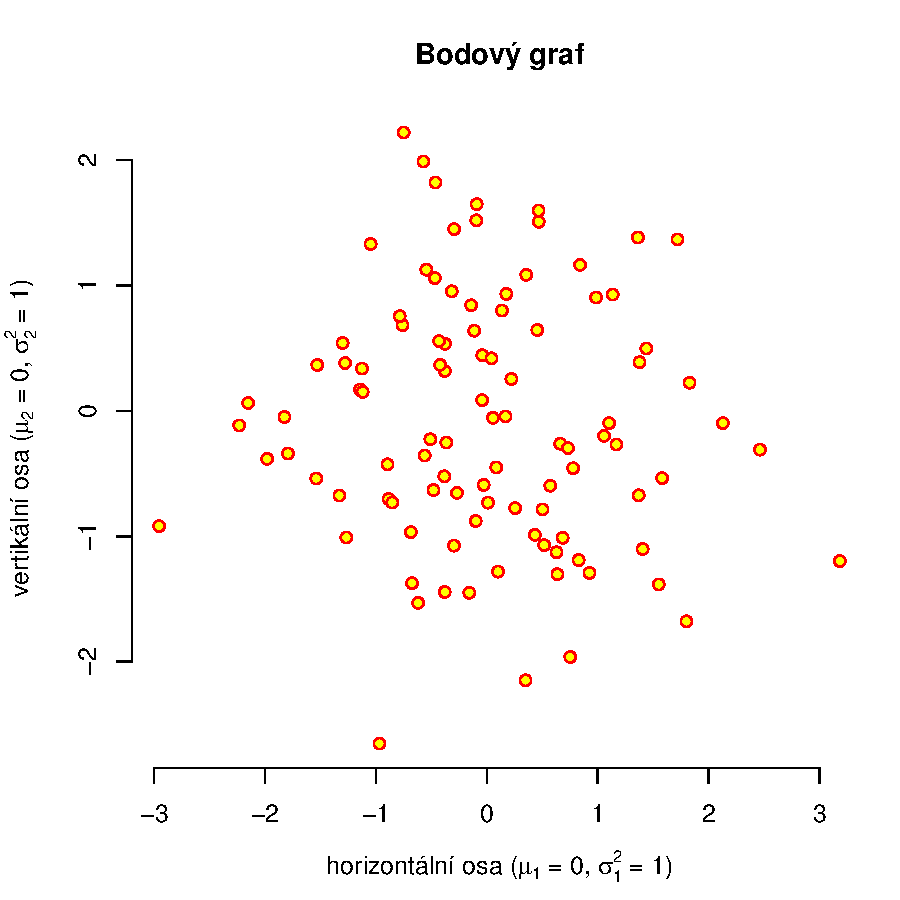
\includegraphics[width=.6\linewidth]{img/ukazka-obr01.pdf}
\caption{This caption is a friendly reminder to never insert figures ``in text,'' without a floating environment, unless explicitly needed for maintaining the text flow (e.g., the figure is small and developing with the text, like some of the centered equations, as in \cref{thm:y}). All figures \emph{must} be referenced by number from the text (so that the readers can find them when they read the text) and properly captioned (so that the readers can interpret the figure even if they look at it before reading the text --- reviewers love to do that).}
\label{fig:f}
\end{figure}

It is sometimes convenient (even recommended by some journals, including Cell) to name the results sub-sections so that they state what exactly has been achieved. Examples follow.

\section{SuperProgram is faster than OldAlgorithm}
\subsection{Scalability estimation}
\subsection{Precision of the results}
\section{Weird theorem is proven by induction}
\section{Amount of code reduced by CodeRedTool}
\subsection{Example}
\subsection{Performance on real codebases}
\section{Graphics and figure quality}

No matter how great the text content of your thesis is, the pictures will always catch the attention first. This creates the very important first impression of the thesis contents and general quality. Crucially, that also decides whether the thesis is later read with joy, or carefully examined with suspicion.

Preparing your thesis in a way such that this first impression gets communicated smoothly and precisely helps both the reviewer and you: the reviewer will not have a hard time understanding what exactly you wanted to convey, and you will get a better grade.

Making the graphics `work for you' involves doing some extra work that is often unexpected. At the same time, you will need to fit into graphics quality constraints and guidelines that are rarely understood before you actually see a bad example. As a rule of thumb, you should allocate at least the same amount of time and effort for making the figures look good as you would for writing, editing and correcting the same page area of paragraph text.

\subsection{Visualize all important ideas}
The set of figures in your thesis should be comprehensive and complete. For all important ideas, constructions, complicated setups and results there should be a visualization that the reader can refer to in case the text does not paint the `mental image' sufficiently well. At the bare minimum, you should have at least 3 figures (roughly corresponding to the 3 chapters) that clearly and unambiguously show:
\begin{enumerate}
\item the context of the problem you are solving, optionally with e.g.~question marks and exclamation marks placed to highlight the problems and research questions
\item the overall architecture of your solution (usually as a diagram with arrows, such as in \cref{fig:schema}, ideally with tiny toy examples of the inputs and outputs of each box),
\item the advancement or the distinctive property of your solution, usually in a benchmark plot, or as a clear demonstration and comparison of your results.
\end{enumerate}

\subsection{Make the figures comprehensible}
The figures should be easily comprehensible. Surprisingly, that requires you to follow some common ``standards'' in figure design and processing. People are often used to a certain form of the visualizations, and (unless you have a very good reason) deviating from the standard is going to make the comprehension much more complicated. The common standards include the following:
\begin{itemize}
  \item caption everything correctly, place the caption at an expectable position
  \item systematically label the plots with `main' titles (usually in boldface, above the plot), plot axes, axis units and ticks, and legends
  \item lay out the diagrams systematically, ideally follow a structure of a bottom-up tree, a left-to-right pipeline, a top-down layered architecture, or a center-to-borders mindmap
  \item {use colors that convey the required information correctly \par\footnotesize Although many people carry some intuition for color use, achieving a really correct utilization of colors is often very hard without previous experience in color science and typesetting. Always remember that everyone perceives color hues differently, therefore the best distinction between the colors is done by varying lightness of the graphics elements (i.e., separating the data by dark vs.~light) rather than by using hues (i.e., forcing people to guess which one of salmon and olive colors means ``better''). Almost 10\% of the population have their vision impaired by some form of color vision deficiency, most frequently by deuteranomaly that prevents interpretation of even the most `obvious' hue differences, such as green vs.~red. Finally, printed colors look surprisingly different from the on-screen colors. You can prevent much of these problems by using standardized palettes and well-tested color gradients, such as the ones from ColorBrewer\footnote{\url{https://colorbrewer2.org}} and ViridisLite\footnote{\url{https://sjmgarnier.github.io/viridisLite/}}. Check if your pictures still look good if converted to greyscale, and use a color deficiency simulator to check how the colors are perceived with deuteranomaly.}
\end{itemize}

Avoid large areas of over-saturated and dark colors:
\begin{itemize}
  \item under no circumstances use dark backgrounds for any graphical elements, such as diagram boxes and tables --- use very light, slightly desaturated colors instead
  \item avoid using figures that contain lots of dark color (as a common example, heatmaps rendered with the `magma' color palette often look like huge black slabs that are visible even through the paper sheet, thus making a dark smudge on the neighboring page)
  \item increase the brightness of any photos to match the average brightness of the text around the figure
\end{itemize}

Remember to test your figures on other people --- usually, just asking `What do you think the figure should show?' can help you debug many mistakes in your graphics. If they think that the figure says something different than what you planned, then most likely it is your figure what is wrong, not the understanding of others.

Finally, there are many magnificent resources that help you arrange your graphics correctly. The two books by Tufte~\cite{tufte1990envisioning,tufte1983visual} are arguably classics in the area. Additionally, you may find many interesting resources to help you with technical aspects of plotting, such as the \texttt{ggplot}-style `Fundamentals' book by~\citet{wilke2019fundamentals}, and a wonderful manual for the TikZ/PGF graphics system by~\citet{tantau2015tikz} that will help you draw high-quality diagrams (like the one in~\cref{fig:schema}).

\section{What is a discussion?}
After you present the results and show that your contributions work, it is important to \emph{interpret} them, showing what they mean in the wider context of the thesis topic, for the researchers who work in the area, and for the more general public, such as for the users.

Separate discussion sections are therefore common in life sciences where some ambiguity in result interpretation is common, and the carefully developed intuition about the wider context is sometimes the only thing that the authors have. Exact sciences and mathematicians do not need to use the discussion sections as often. Despite of that, it is nice to position your output into the previously existing environment, answering:
\begin{itemize}
\item What is the potential application of the result?
\item Does the result solve a problem that other people encountered?
\item Did the results point to any new (surprising) facts?
\item How (and why) is the approach you chose different from what the others have done previously?
\item Why is the result important for your future work (or work of anyone other)?
\item Can the results be used to replace (and improve) anything that is used currently?
\end{itemize}

If you do not know the answers, you may want to ask the supervisor. Also, do not worry if the discussion section is half-empty or completely pointless; you may remove it completely without much consequence. It is just a bachelor thesis, not a world-saving avenger thesis.


\chapwithtoc{Conclusion}

\xxx{TODO: add conclusion}

In the conclusion, you should summarize what was achieved by the thesis. In a few paragraphs, try to answer the following:
\begin{itemize}
\item Was the problem stated in the introduction solved? (Ideally include a list of successfully achieved goals.)
\item What is the quality of the result? Is the problem solved for good and the mankind does not need to ever think about it again, or just partially improved upon? (Is the incompleteness caused by overwhelming problem complexity that would be out of thesis scope\todo{This is quite common.}, or any theoretical reasons, such as computational hardness?)
\item Does the result have any practical applications that improve upon something realistic?
\item Is there any good future development or research direction that could further improve the results of this thesis? (This is often summarized in a separate subsection called `Future work'.)
\end{itemize}


\ifEN
\chapwithtoc{Bibliography}
\else
\chapwithtoc{Seznam použité literatury}
\fi

\printbibliography[heading=none]


\appendix
\chapter{Using CoolThesisSoftware}

Use this appendix to tell the readers (specifically the reviewer) how to use your software. A very reduced example follows; expand as necessary. Description of the program usage (e.g., how to process some example data) should be included as well.

To compile and run the software, you need dependencies XXX and YYY and a C compiler. On Debian-based Linux systems (such as Ubuntu), you may install these dependencies with APT:
\begin{Verbatim}
apt-get install \
  libsuperdependency-dev \
  libanotherdependency-dev \
  build-essential
\end{Verbatim}

To unpack and compile the software, proceed as follows:
\begin{Verbatim}
unzip coolsoft.zip
cd coolsoft
./configure
make
\end{Verbatim}

The program can be used as a C++ library, the simplest use is demonstrated in \cref{lst:ex}. A demonstration program that processes demonstration data is available in directory \verb|demo/|, you can run the program on a demonstration dataset as follows:
\begin{Verbatim}
cd demo/
./bin/cool_process_data data/demo1
\end{Verbatim}

After the program starts, control the data avenger with standard \verb-WSAD- controls.

\begin{listing}
\begin{lstlisting}
#include <CoolSoft.h>
#include <iostream>

int main() {
	int i;
	if(i = cool::ProcessAllData()) // returns 0 on error
		std::cout << i << std::endl;
	else
		std::cerr << "error!" << std::endl;
	return 0;
}
\end{lstlisting}
\caption{Example program.}
\label{lst:ex}
\end{listing}


% if your attachments are complicated, describe them in a separate appendix
%\include{attachments}

\openright
\end{document}
